\documentclass{beamer}
\usetheme{metropolis}

% specifications for presenter mode
%\beamerdefaultoverlayspecification{<+->}
%\setbeamercovered{transparent}

\usepackage[english]{babel}
\usepackage[utf8x]{inputenc}

%\usepackage{coloremoji}
\usepackage{layout}
\usepackage{multirow}
\usepackage{array}
\usepackage{graphicx}
\graphicspath{ {figs/} }

\setbeameroption{hide notes}
\setbeamertemplate{note page}[plain]
\usepackage{listings}
\usepackage{datetime}
\usepackage{url}
\usepackage{tcolorbox}
\usepackage{appendixnumberbeamer}

\usepackage{tikz}
\def\checkmark{\tikz\fill[scale=0.4](0,.35) -- (.25,0) -- (1,.7) -- (.25,.15) -- cycle;}

% math shorthand
\usepackage{bm}
\usepackage{amstext}
\usepackage{amsthm}
\usepackage{amsmath}
\usepackage{mathtools}
\newcommand{\R}{\mathbb{R}}
\newcommand{\D}{\mathcal{D}}
\newcommand{\E}{\mathbb{E}}
\newcommand{\I}{\mathbb{I}}
\newcommand{\pr}{\mathbb{P}}
\newcommand{\F}{\mathcal{F}}
\newcommand{\X}{\mathcal{X}}
\newcommand{\M}{\mathcal{M}}
\newcommand{\lik}{\mathcal{L}}

\newtheorem*{assumption*}{\assumptionnumber}
\providecommand{\assumptionnumber}{}
\makeatletter
\newenvironment{assumption}[2]
 {%
  \renewcommand{\assumptionnumber}{Assumption #1: $\mathcal{#2}$}%
  \begin{assumption*}%
  \protected@edef\@currentlabel{#1: $\mathcal{#2}$}%
 }
 {%
  \end{assumption*}
 }
\makeatother

\DeclarePairedDelimiterX{\infdivx}[2]{(}{)}{%
  #1\;\delimsize\|\;#2%
}
\newcommand{\infdiv}{D\infdivx}
\DeclarePairedDelimiter{\norm}{\lVert}{\rVert}
\DeclareMathOperator*{\argmin}{arg\,min}
\DeclareMathOperator*{\argmax}{arg\,max}

% indepndence notation macro
\newcommand\indep{\protect\mathpalette{\protect\independenT}{\perp}}
\def\independenT#1#2{\mathrel{\rlap{$#1#2$}\mkern2mu{#1#2}}}

% Bibliography
\usepackage{natbib}
\bibpunct{(}{)}{,}{a}{}{;}
\usepackage{bibentry}

% title info
\title{\normalsize Leveraging the causal effects of stochastic interventions to
  evaluate vaccine efficacy in two-phase trials}

\author{\href{https://nimahejazi.org}{Nima Hejazi}\\[-10pt]}

\institute{
  \begin{figure}[!htb]
    \centering
    \begin{minipage}{.65\textwidth}
        Division of Biostatistics, and \\
        Center for Computational Biology, \\
        University of California, Berkeley \\[6pt]
        
\includegraphics[scale=0.12]{twitter-icon.png}
          \href{https://twitter.com/nshejazi}{nshejazi} \\
        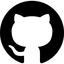
\includegraphics[scale=0.09]{github-icon.png}
          \href{https://github.com/nhejazi}{nhejazi} \\
        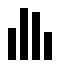
\includegraphics[scale=0.12]{homepage.png}
          \href{https://nimahejazi.org}{nimahejazi.org} \\
      with D.~Benkeser, M.~van der Laan, H.~Janes, P.~Gilbert\\
    SER: ``Methods for the thorny challenges of real studies''
    \end{minipage}%
    \begin{minipage}{0.35\textwidth}
      \centering
      
\includegraphics[height=0.80in,width=0.80in]{ucberkeleyseal_874_540.eps}
    \end{minipage}
  \end{figure}
}

\date{}
%\date{Wednesday, 16 December 2020}

%%%%%%%%%%%%%%%%%%%%%%%%%%%%%%%%%%%%%%%%%%%%%%%%%%%%%%%%%%%%%%%%%%%%%%%%%%%%%%%%

% Outline at beginning of each section
%\AtBeginSection[]
%{
  %\begin{frame}<beamer>
    %\frametitle{Outline}
    %\tableofcontents[currentsection]
  %\end{frame}
%}

%%%%%%%%%%%%%%%%%%%%%%%%%%%%%%%%%%%%%%%%%%%%%%%%%%%%%%%%%%%%%%%%%%%%%%%%%%%%%%%%

\begin{document}

\begin{frame}[noframenumbering]
  \thispagestyle{empty}
  \titlepage
\end{frame}

%%%%%%%%%%%%%%%%%%%%%%%%%%%%%%%%%%%%%%%%%%%%%%%%%%%%%%%%%%%%%%%%%%%%%%%%%%%%%%%%

\begin{frame}[c]{The burden of HIV-1}

\begin{center}
\begin{itemize}
  \itemsep10pt
  \item The HIV-1 epidemic --- the facts:
    \begin{itemize}
      \item now in its fourth decade,
      \item 2.5 million new infections occurring annually worldwide,
      \item new infections outpace patients starting antiretroviral therapy.
    \end{itemize}
  \item \textit{Most efficacious} preventive vaccine: 31\% reduction rate.
  \item \textbf{Question}: To what extent can HIV-1 vaccines be improved by
    modulating immunogenic CD4+/CD8+ response profiles?
\end{itemize}
\end{center}

\note{
}

\end{frame}

%%%%%%%%%%%%%%%%%%%%%%%%%%%%%%%%%%%%%%%%%%%%%%%%%%%%%%%%%%%%%%%%%%%%%%%%%%%%%%%%
\begin{frame}[c]{HVTN 505 trial examined new antibody boost vaccines}

\begin{center}
\begin{itemize}
  \itemsep10pt
  \item HIV Vaccine Trials Network's (HVTN) 505 vaccine efficacy; randomized
    controlled trial, $n = 2504$ \citep{hammer2013efficacy}.
  \item Immunogenic response profiles only available for two-phase sample of
    $n = 189$ \citep{janes2017higher} due to cost limitations.
  \item \underline{Two-phased sampling mechanism:} 100\% inclusion rate if
    HIV-1 positive in week 28; based on matching otherwise.
  \item \textbf{Question:} How would HIV-1 infection risk in week 28 have
    changed had immunogenic response (due to vaccine) differed?
\end{itemize}
\end{center}

\note{
\begin{itemize}
  \itemsep10pt
  \item Baseline covariates($L$): sex, age, BMI, behavioral HIV risk.
  \item Intervention(s) ($A$): post-vaccination T-cell activity markers.
  \item Outcome ($Y$): HIV-1 infection status at week 28 of tiral.
  \item 12-color intracellular cytokine staining (ICS) assay.
  \item Cryopreserved peripheral blood mononuclear cells were stimulated with
    synthetic HIV-1 peptide pools.
  \item All immune responses are assayed \textit{after} the endpoints of
    interest (HIV-1 infection status) are collected.
  \item \textbf{Conclusion:} Understanding which immune responses impact vaccine
    efficacy helps develop more efficacious vaccines.
  \item A vaccine effective at preventing HIV-1 acquisition would be a
    cost-effective and durable approach to halting the worldwide epidemic.
  \item Identifying vaccine-induced immune-response biomarkers that predict a
    vaccine's ability to protect individuals from HIV-1 infection is a high
    priority.
  \item The study was halted on 22 April 2013 due to absence of vaccine
    efficacy. There was no significant effect of the vaccine on the primary
    infection endpoint of HIV-1 infection between week 28 and month 24.
\end{itemize}
}

\end{frame}

%%%%%%%%%%%%%%%%%%%%%%%%%%%%%%%%%%%%%%%%%%%%%%%%%%%%%%%%%%%%%%%%%%%%%%%%%%%%%%%%

\begin{frame}[c]{Two-phase sampling censors the complete data structure}

\begin{center}
\begin{itemize}
  \itemsep10pt
  \item Complete (\underline{unobserved}) data $X = (L, A, Y) \sim P_0^X \in
    \mathcal{M}^X$, as per the full HVTN 505 trial cohort
    \citep{hammer2013efficacy}:
    \vspace{1em}
    \begin{itemize}
      \itemsep8pt
      \item $L$ (baseline covariates): sex, age, BMI, behavioral HIV risk;
      \item $A$ (exposure): immunogenic response profiles (CD4+, CD8+);
      \item $Y$ (outcome of interest): HIV-1 infection status at week 28.
    \end{itemize}
  \item Observed data $O = (C, C X) = (L, C, C A, Y)$; $C \in \{0,1\}$ is an
    indicator for inclusion in the two-phase sample.
  \item Can we use the two-phase sample ($n = 189$) to estimate causal effects
    in the vaccine arm ($n \approx 1400$)? How?
\end{itemize}
\end{center}

\note{
  \begin{itemize}
    \item $P_0^X$ --- true (unknown) distribution of the full data $X$.
    \item $\mathcal{M}^X_{NP}$ --- nonparametric statistical model.
    \item Observed data $O$ is a masked version of the full data $X$.
  \end{itemize}
}

\end{frame}

%%%%%%%%%%%%%%%%%%%%%%%%%%%%%%%%%%%%%%%%%%%%%%%%%%%%%%%%%%%%%%%%%%%%%%%%%%%%%%%%

\begin{frame}[c]{Stochastic interventions define the causal effects of shifts}

\begin{center}
\begin{itemize}
  \itemsep10pt
  \item Causal estimand: counterfactual mean of HIV-1 infection under a
    \textit{shifted} immunogenic response distribution.
  \item \cite{diaz2012population, diaz2018stochastic}: \textit{Shift}
    interventions?
     \begin{equation*}\label{shift_intervention}
       d(a, l) =
         \begin{cases}
           a + \delta, & \text{if plausible} \\
           a, & \text{otherwise}
         \end{cases}
     \end{equation*}
  \item \cite{diaz2012population, diaz2018stochastic} give a statistical target
    parameter and influence function for the complete data case.
  %\item \textbf{Challenge:} parameter estimation requires conditional density
    %estimation. Nonparametric options?
\end{itemize}
\end{center}

\note{
  \begin{itemize}
    \item For HVTN 505, $\psi_{0,d}$ is the counterfactual risk of HIV-1
      infection, had the observed value of the immune response been modifed to
      originate from the distribution of the rule $d(A,W)$.
    \item Several different ways to consider stochastic interventions.
    \item Starts with Mark and Ivan's simple stochastic shift.
    \item Extensions to modified treatment policies.
    \item The new value of $A$ may be denoted $A^* \sim G^*(\cdot \mid W)$,
      where $A^* = d(W, U^*)$ for a rule $d$ and random error $U^*$.
  \end{itemize}
}

\end{frame}

%%%%%%%%%%%%%%%%%%%%%%%%%%%%%%%%%%%%%%%%%%%%%%%%%%%%%%%%%%%%%%%%%%%%%%%%%%%%%%%%

\begin{frame}[c]{HIV-1 risk under shifted immunogenic responses}

%\centering
\hspace*{-1cm}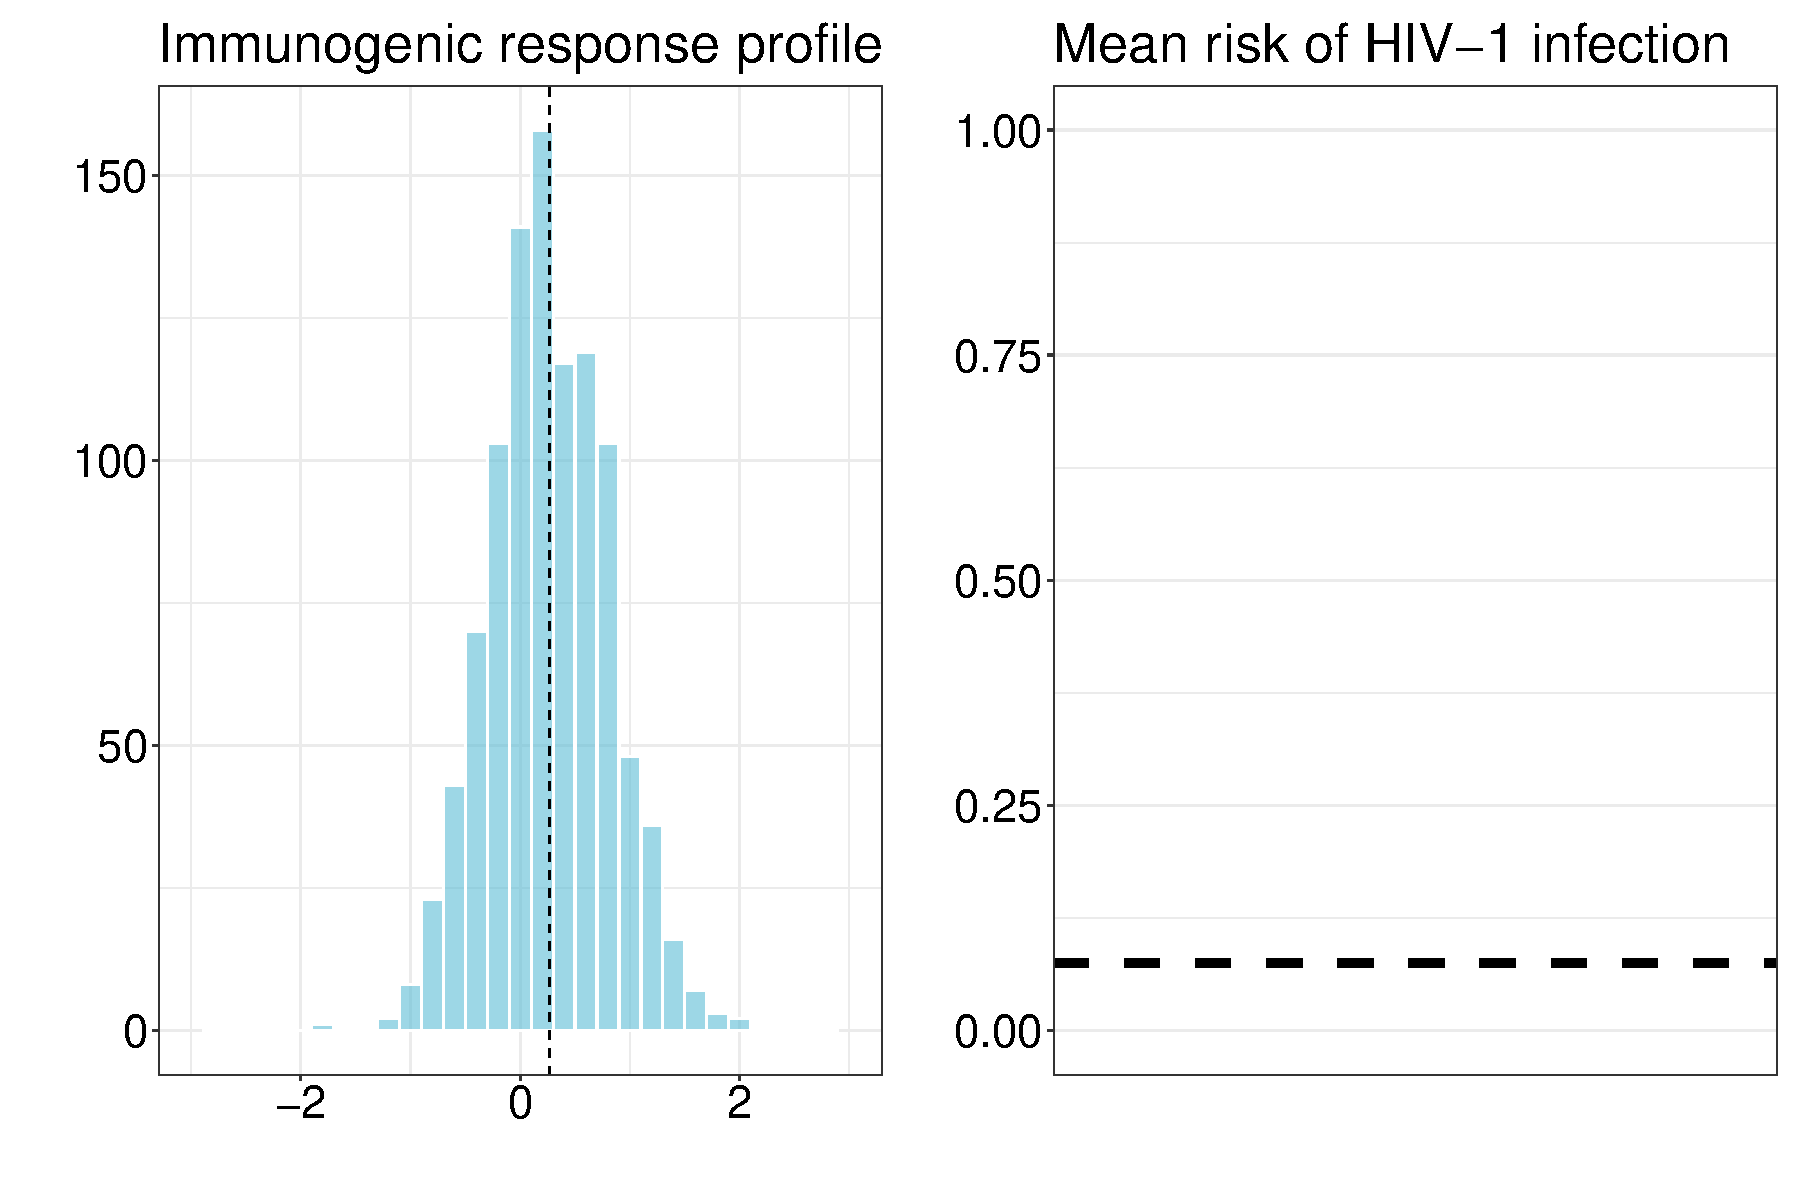
\includegraphics[scale=0.4]{shift-1}

\note{
}

\end{frame}

%%%%%%%%%%%%%%%%%%%%%%%%%%%%%%%%%%%%%%%%%%%%%%%%%%%%%%%%%%%%%%%%%%%%%%%%%%%%%%%%

\begin{frame}[c,noframenumbering]{HIV-1 risk under shifted immunogenic responses}

%\centering
\hspace*{-1cm}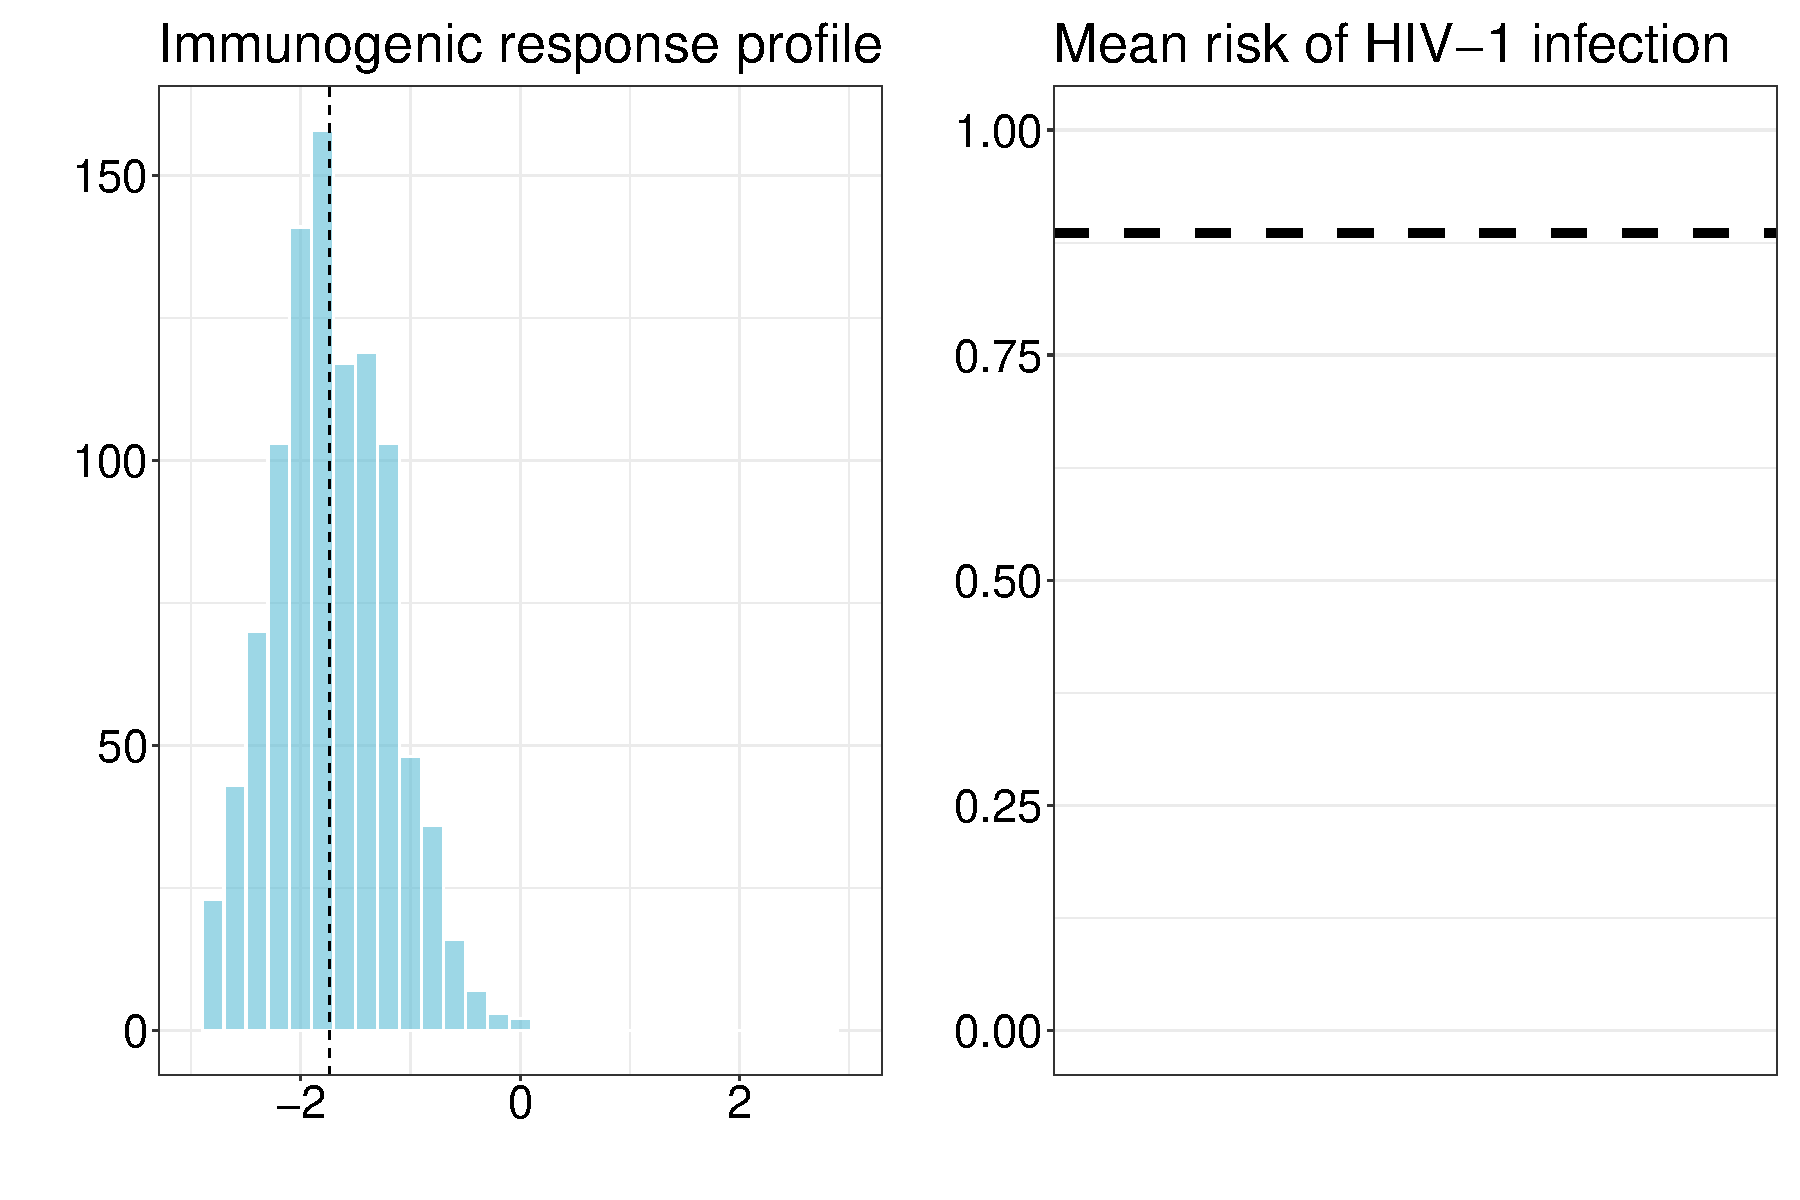
\includegraphics[scale=0.4]{shift-2}

\note{
}

\end{frame}

%%%%%%%%%%%%%%%%%%%%%%%%%%%%%%%%%%%%%%%%%%%%%%%%%%%%%%%%%%%%%%%%%%%%%%%%%%%%%%%%

\begin{frame}[c,noframenumbering]{HIV-1 risk under shifted immunogenic responses}

%\centering
\hspace*{-1cm}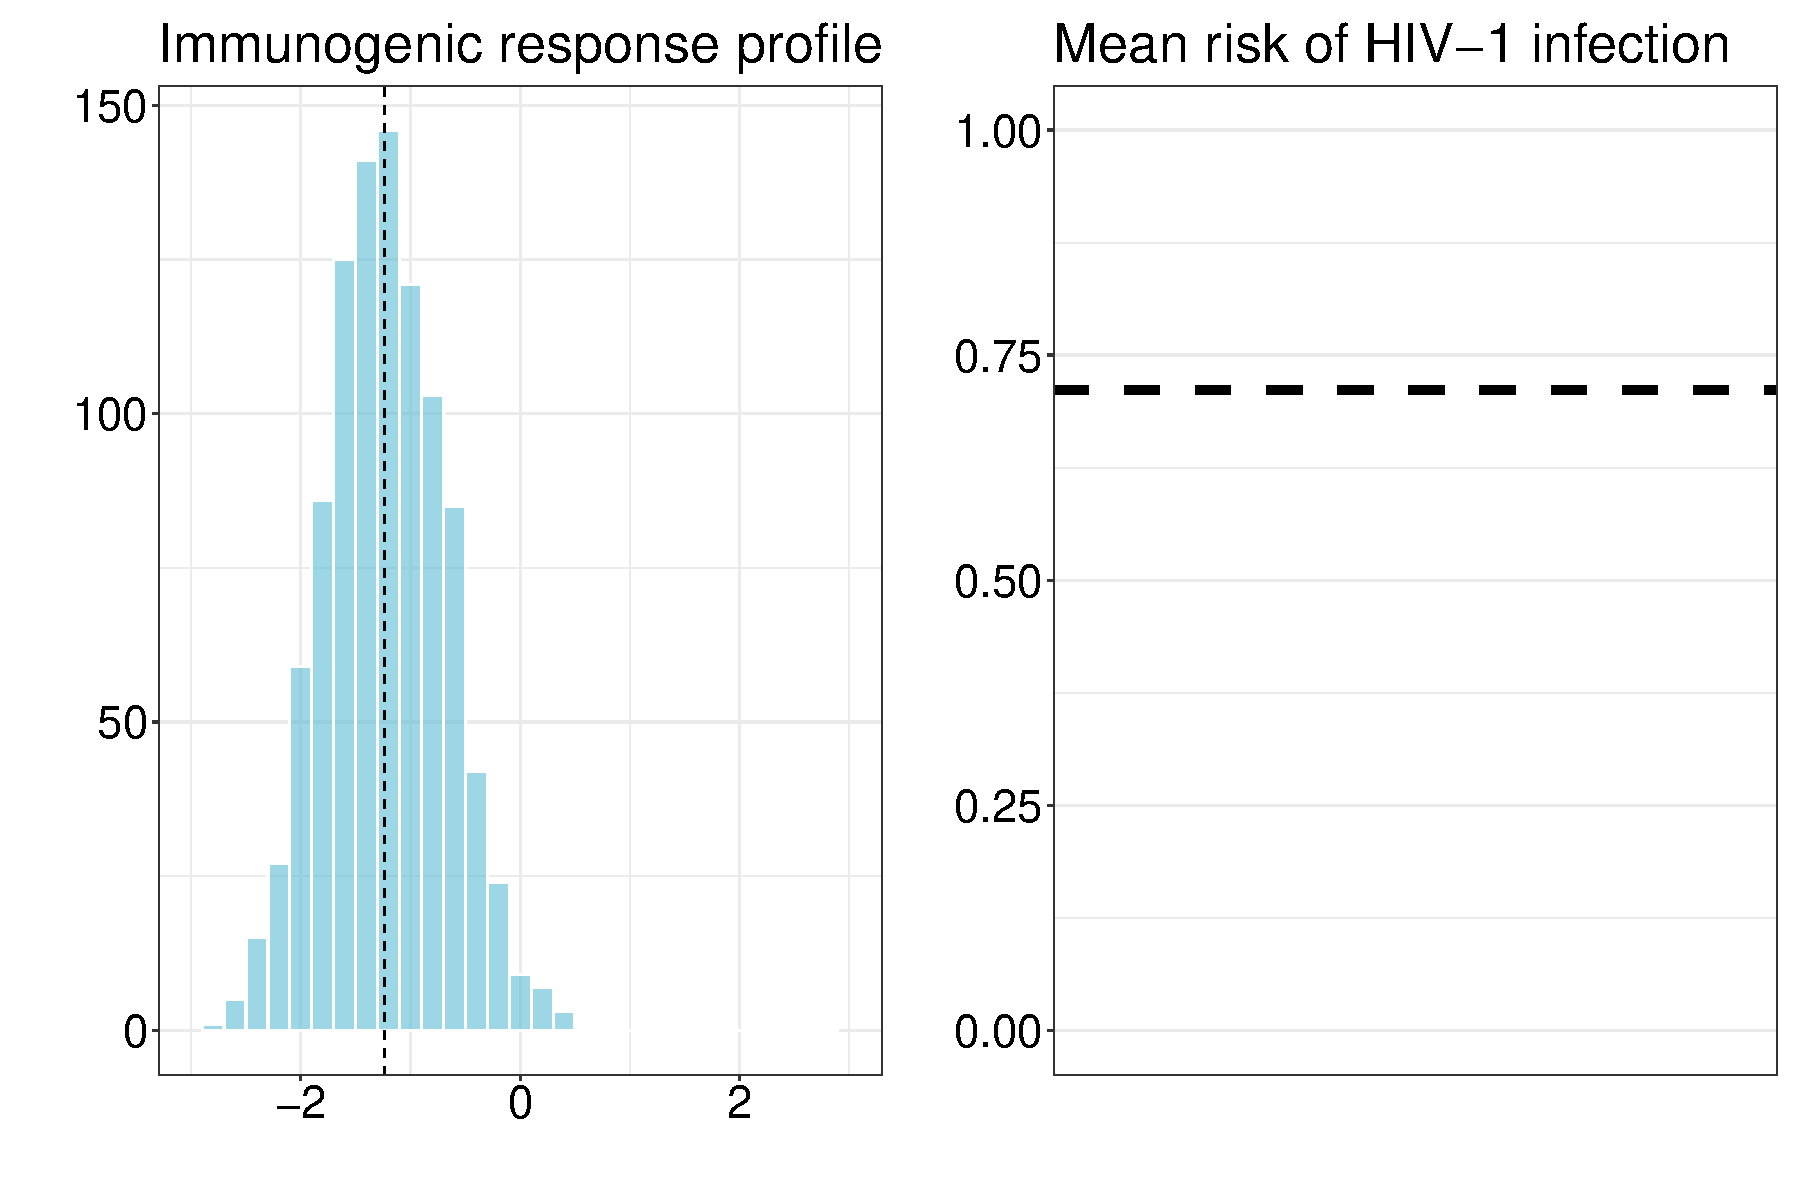
\includegraphics[scale=0.4]{shift-3}

\note{
}

\end{frame}

%%%%%%%%%%%%%%%%%%%%%%%%%%%%%%%%%%%%%%%%%%%%%%%%%%%%%%%%%%%%%%%%%%%%%%%%%%%%%%%%

\begin{frame}[c,noframenumbering]{HIV-1 risk under shifted immunogenic responses}

%\centering
\hspace*{-1cm}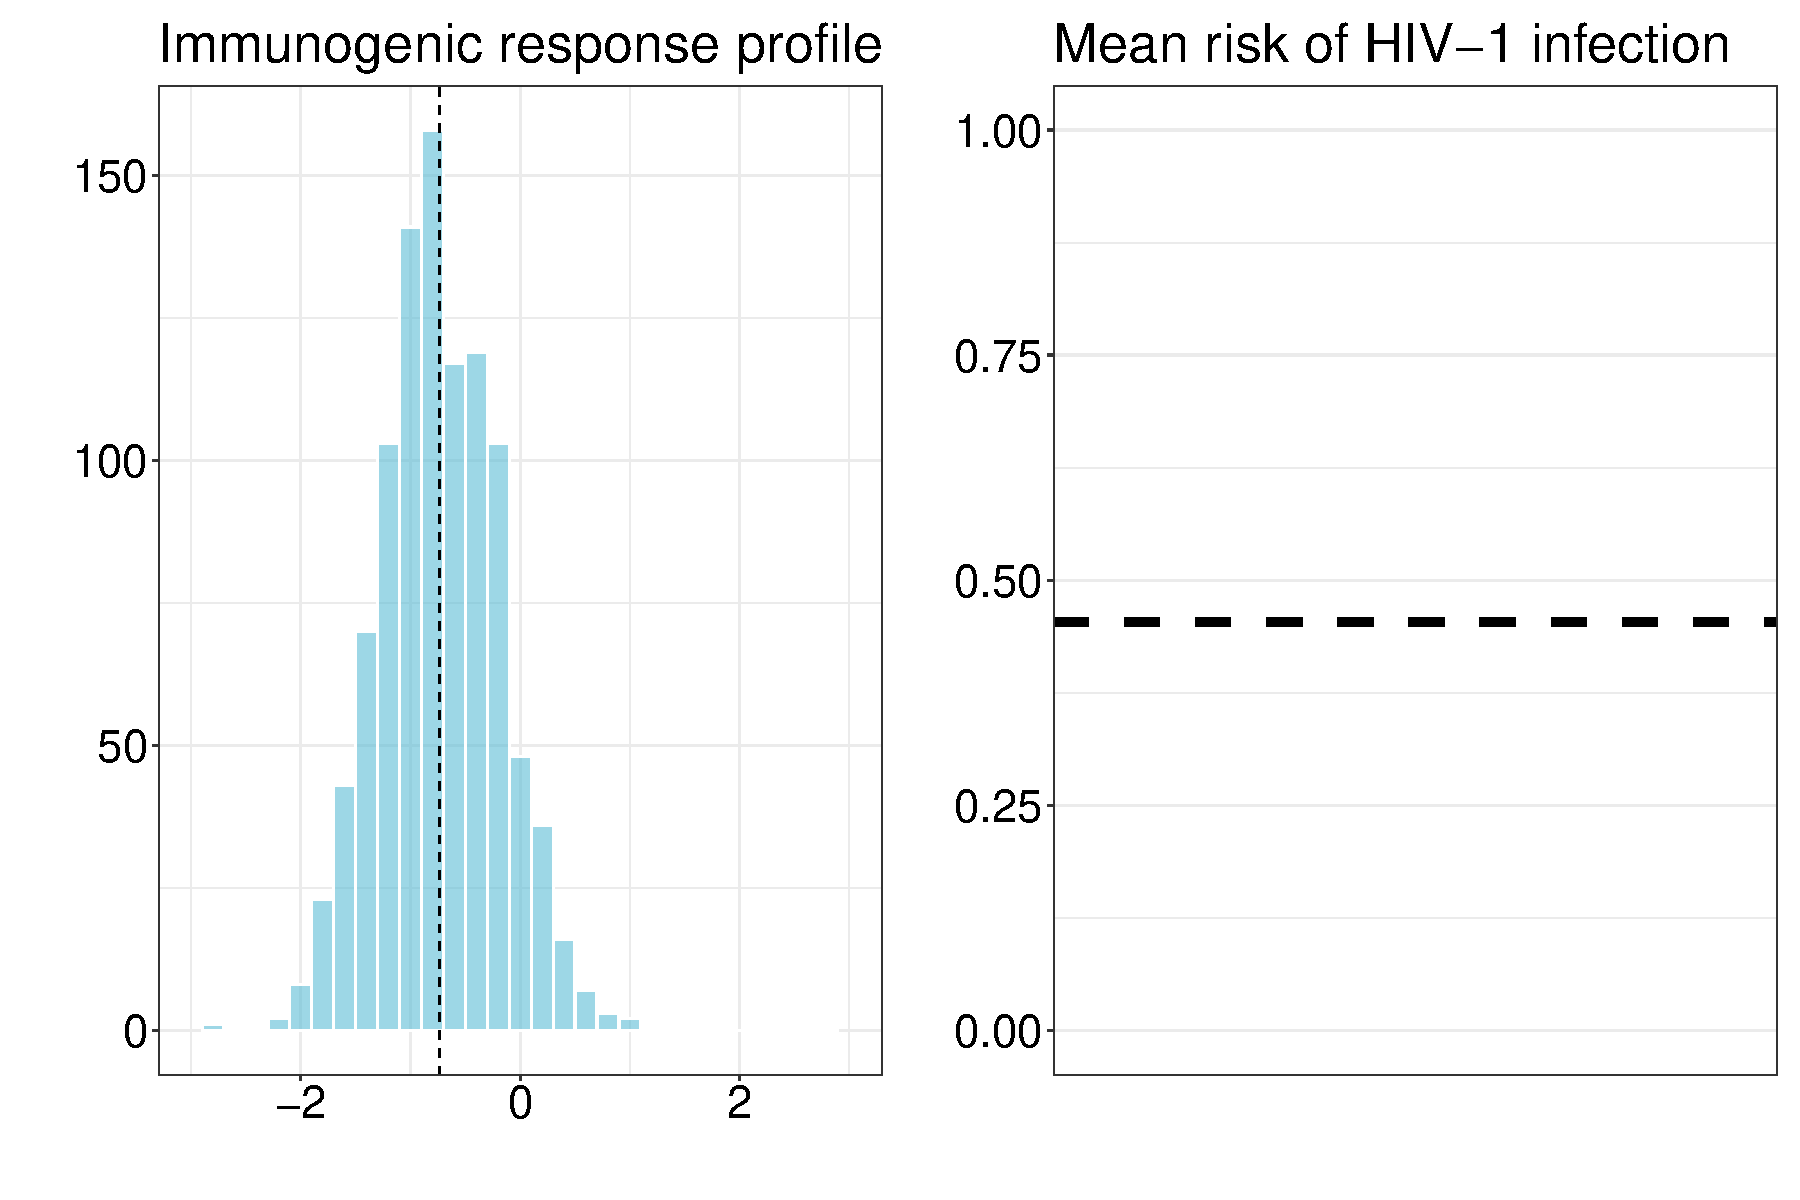
\includegraphics[scale=0.4]{shift-4}

\note{
}

\end{frame}

%%%%%%%%%%%%%%%%%%%%%%%%%%%%%%%%%%%%%%%%%%%%%%%%%%%%%%%%%%%%%%%%%%%%%%%%%%%%%%%%

\begin{frame}[c,noframenumbering]{HIV-1 risk under shifted immunogenic responses}

%\centering
\hspace*{-1cm}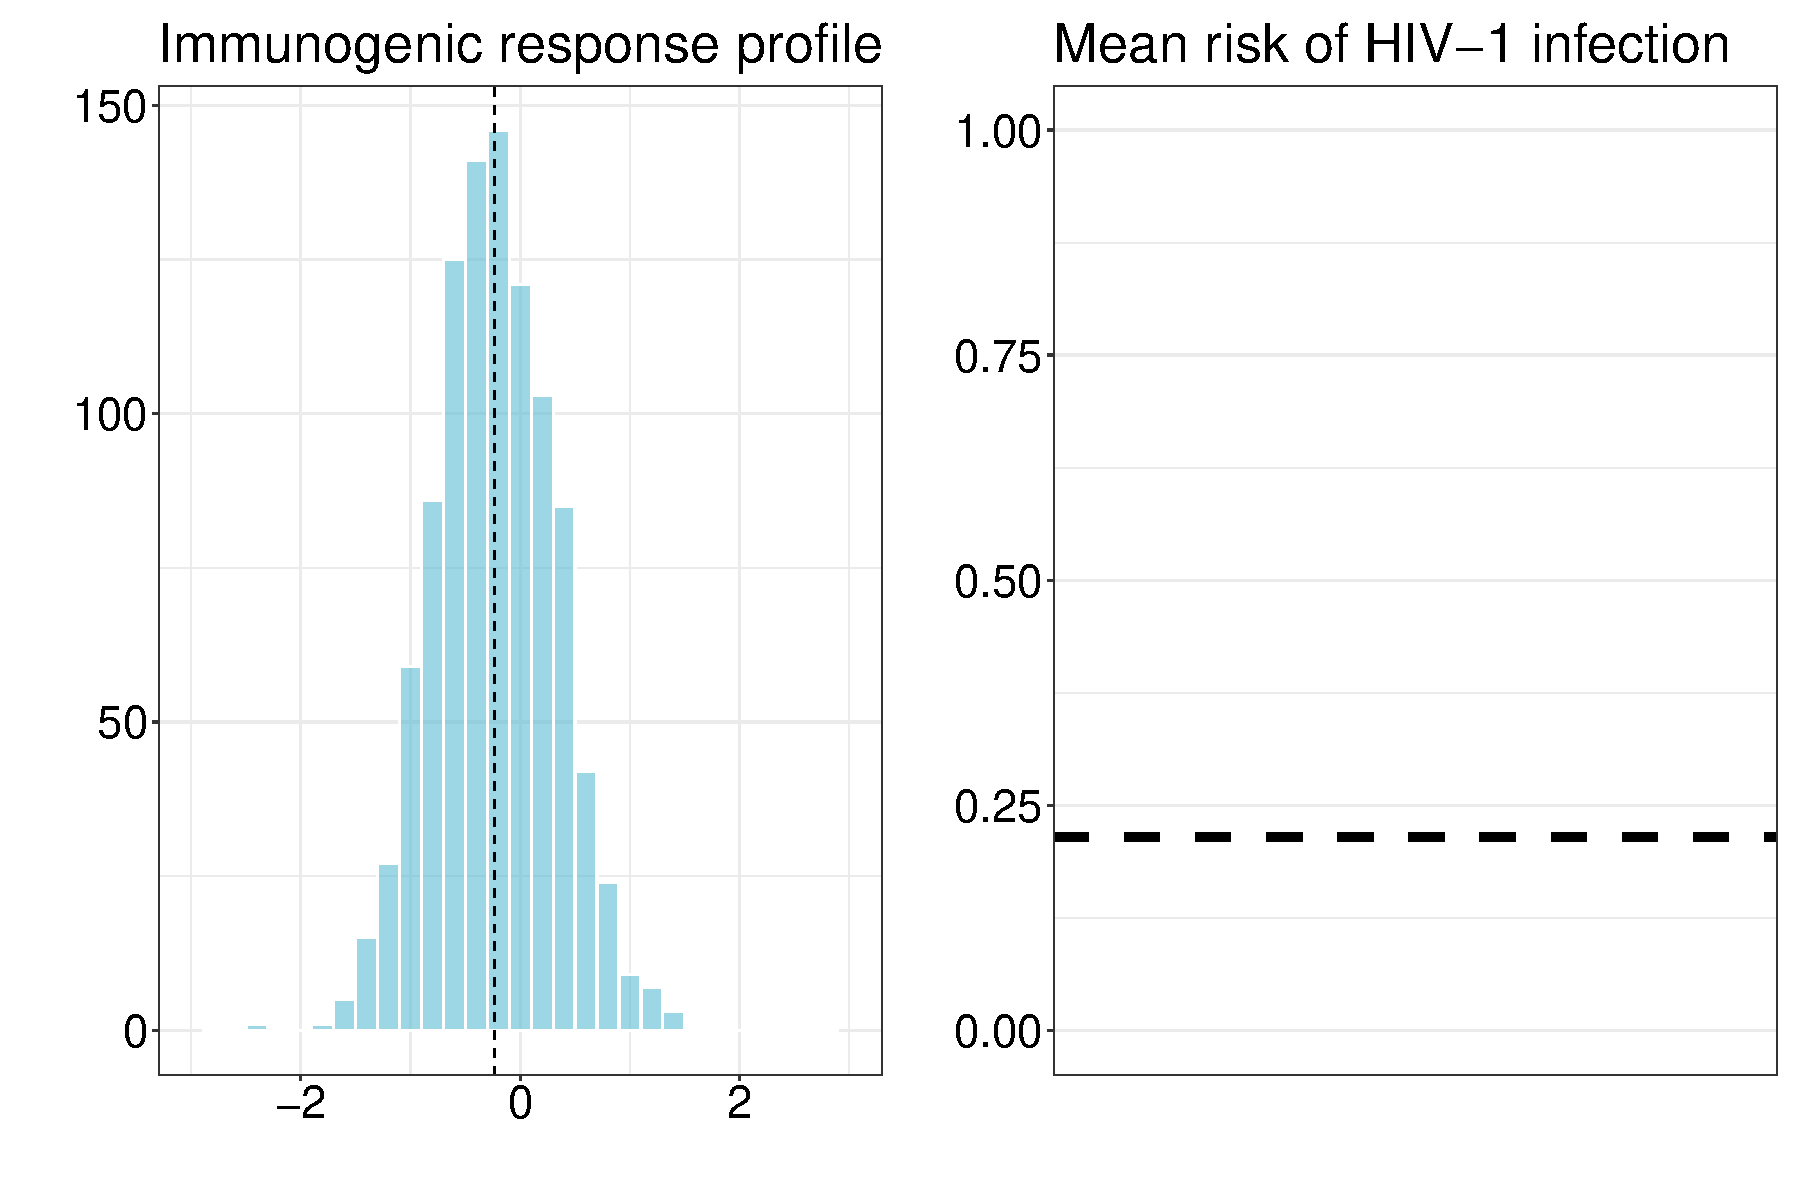
\includegraphics[scale=0.4]{shift-5}

\note{
}

\end{frame}

%%%%%%%%%%%%%%%%%%%%%%%%%%%%%%%%%%%%%%%%%%%%%%%%%%%%%%%%%%%%%%%%%%%%%%%%%%%%%%%%

\begin{frame}[c,noframenumbering]{HIV-1 risk under shifted immunogenic responses}

%\centering
\hspace*{-1cm}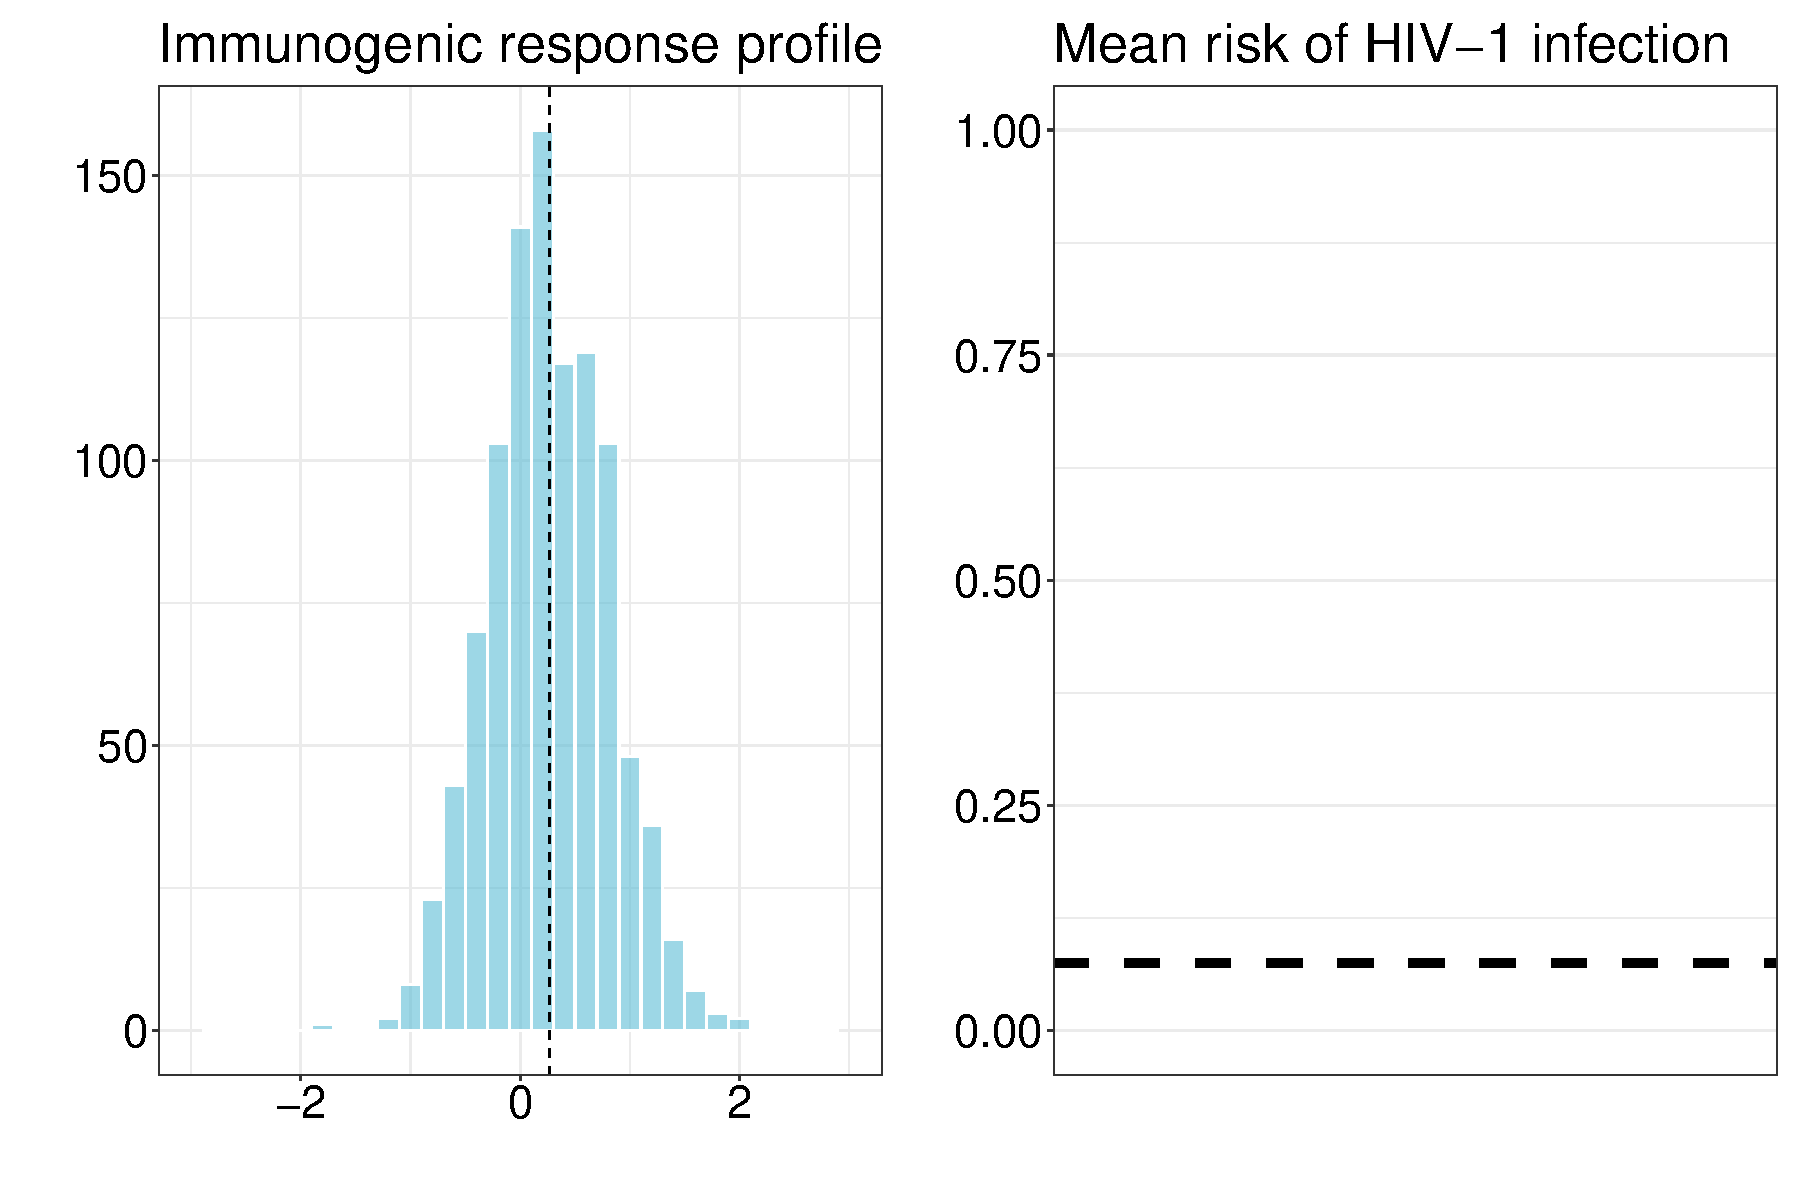
\includegraphics[scale=0.4]{shift-6}

\note{
}

\end{frame}

%%%%%%%%%%%%%%%%%%%%%%%%%%%%%%%%%%%%%%%%%%%%%%%%%%%%%%%%%%%%%%%%%%%%%%%%%%%%%%%%

\begin{frame}[c,noframenumbering]{HIV-1 risk under shifted immunogenic responses}

%\centering
\hspace*{-1cm}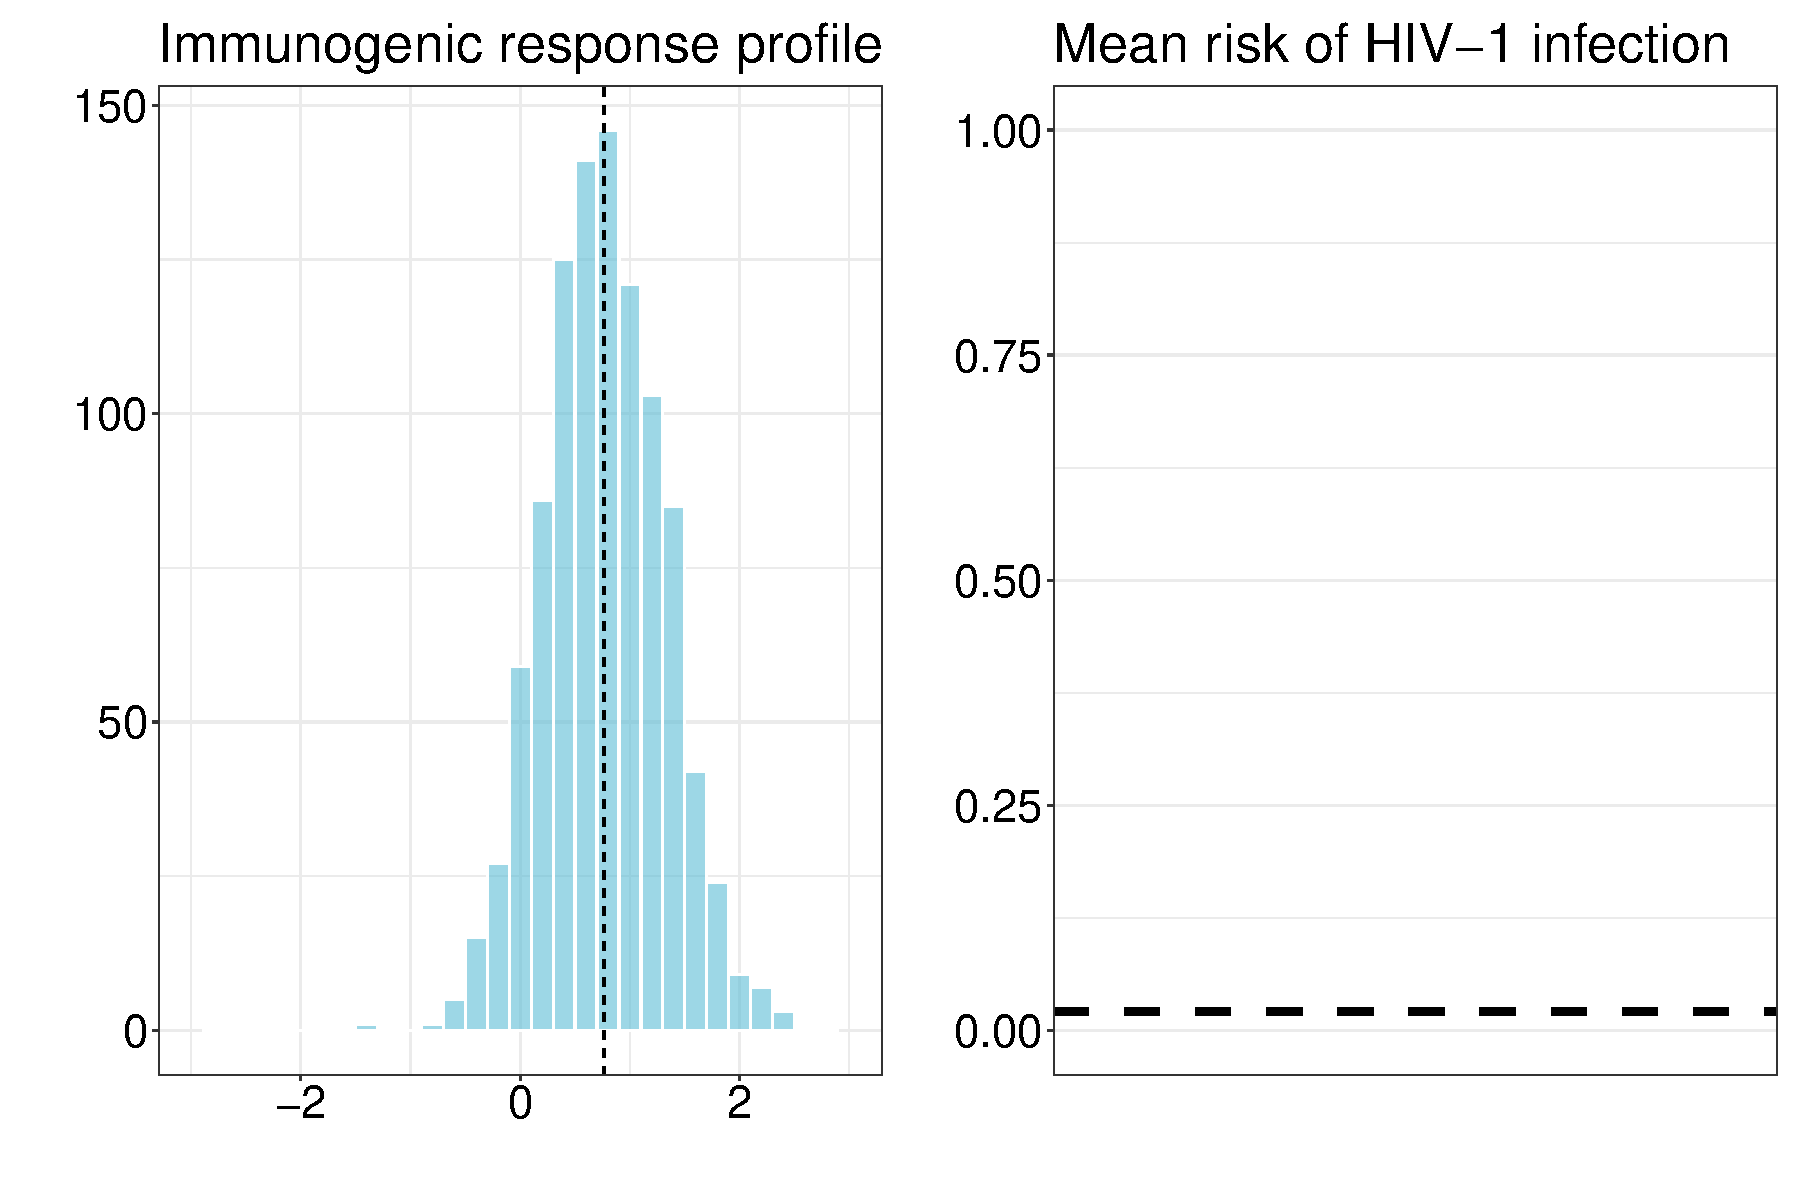
\includegraphics[scale=0.4]{shift-7}

\note{
}

\end{frame}

%%%%%%%%%%%%%%%%%%%%%%%%%%%%%%%%%%%%%%%%%%%%%%%%%%%%%%%%%%%%%%%%%%%%%%%%%%%%%%%%

\begin{frame}[c,noframenumbering]{HIV-1 risk under shifted immunogenic responses}

%\centering
\hspace*{-1cm}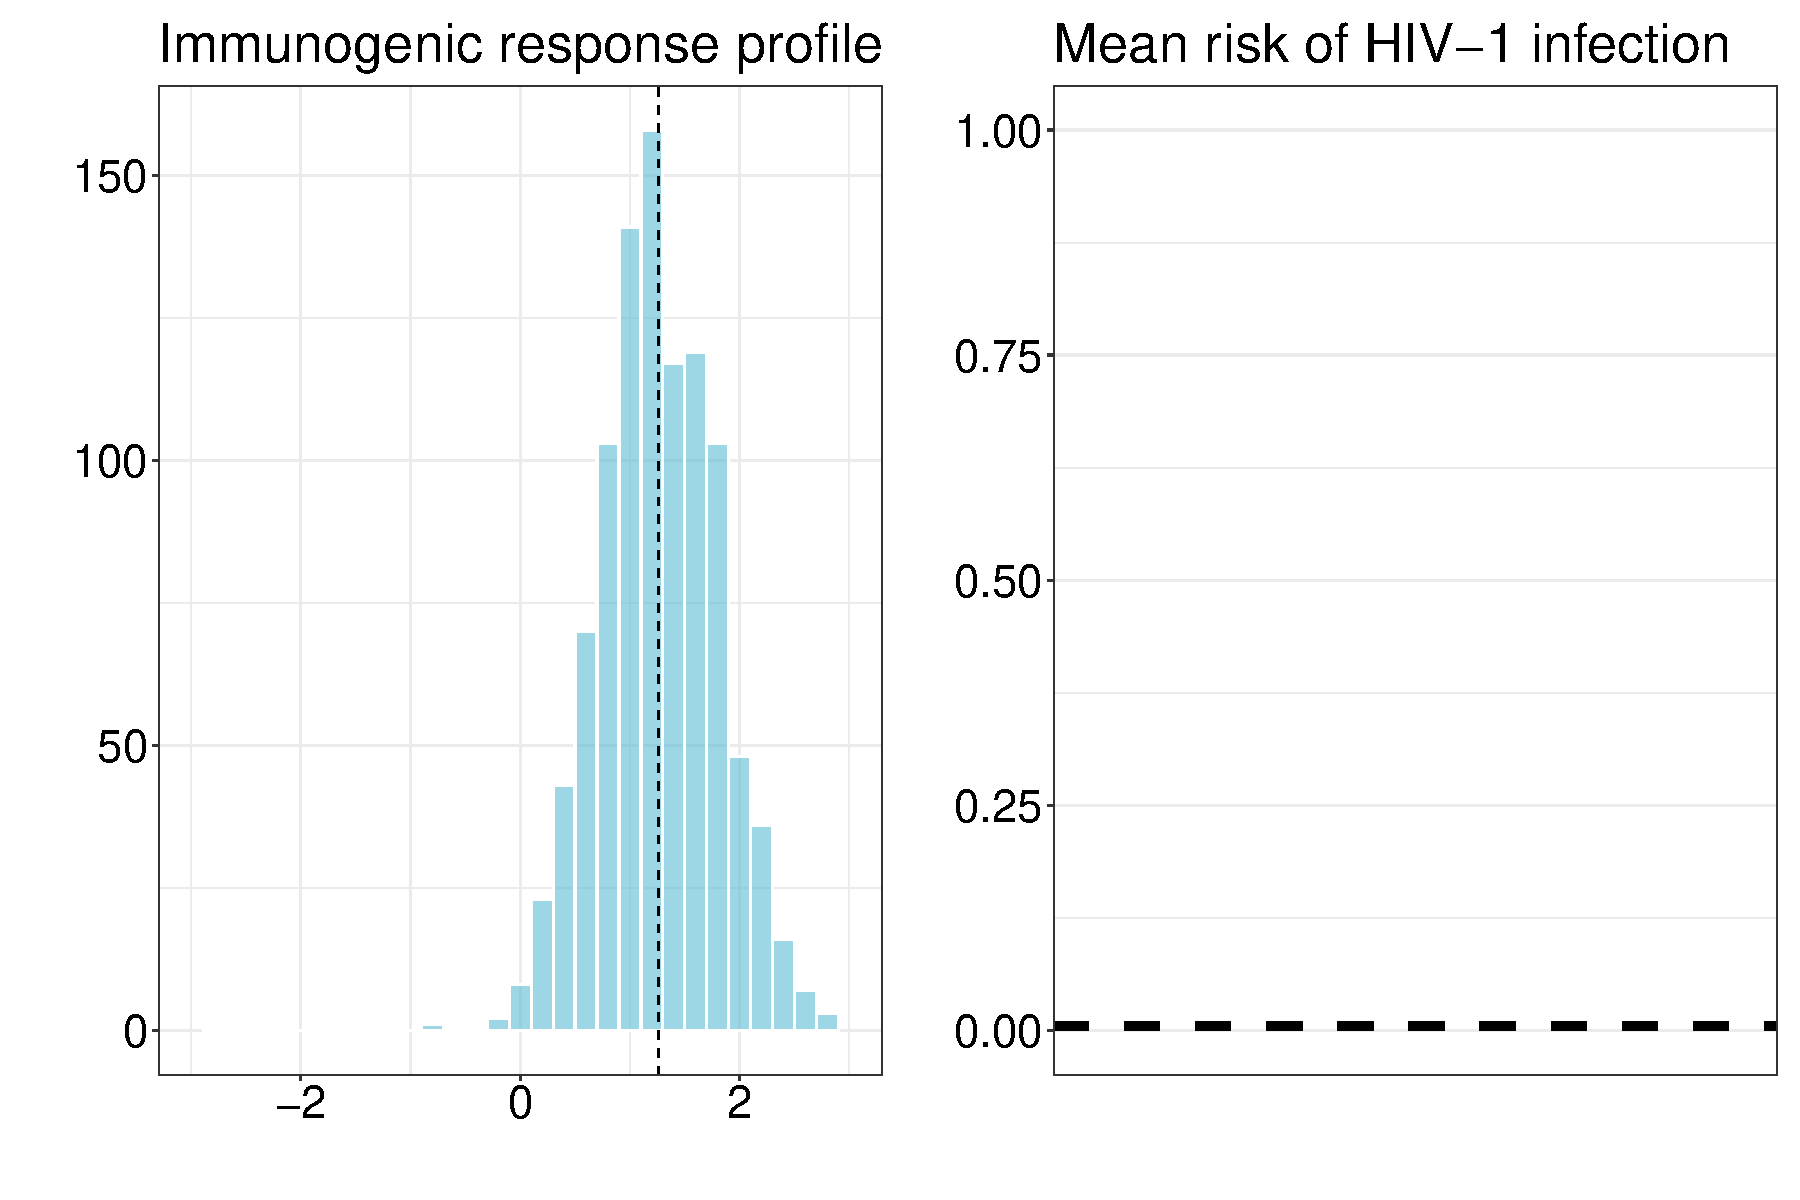
\includegraphics[scale=0.4]{shift-8}

\note{
}

\end{frame}

%%%%%%%%%%%%%%%%%%%%%%%%%%%%%%%%%%%%%%%%%%%%%%%%%%%%%%%%%%%%%%%%%%%%%%%%%%%%%%%%

\begin{frame}[c,noframenumbering]{HIV-1 risk under shifted immunogenic responses}

%\centering
\hspace*{-1cm}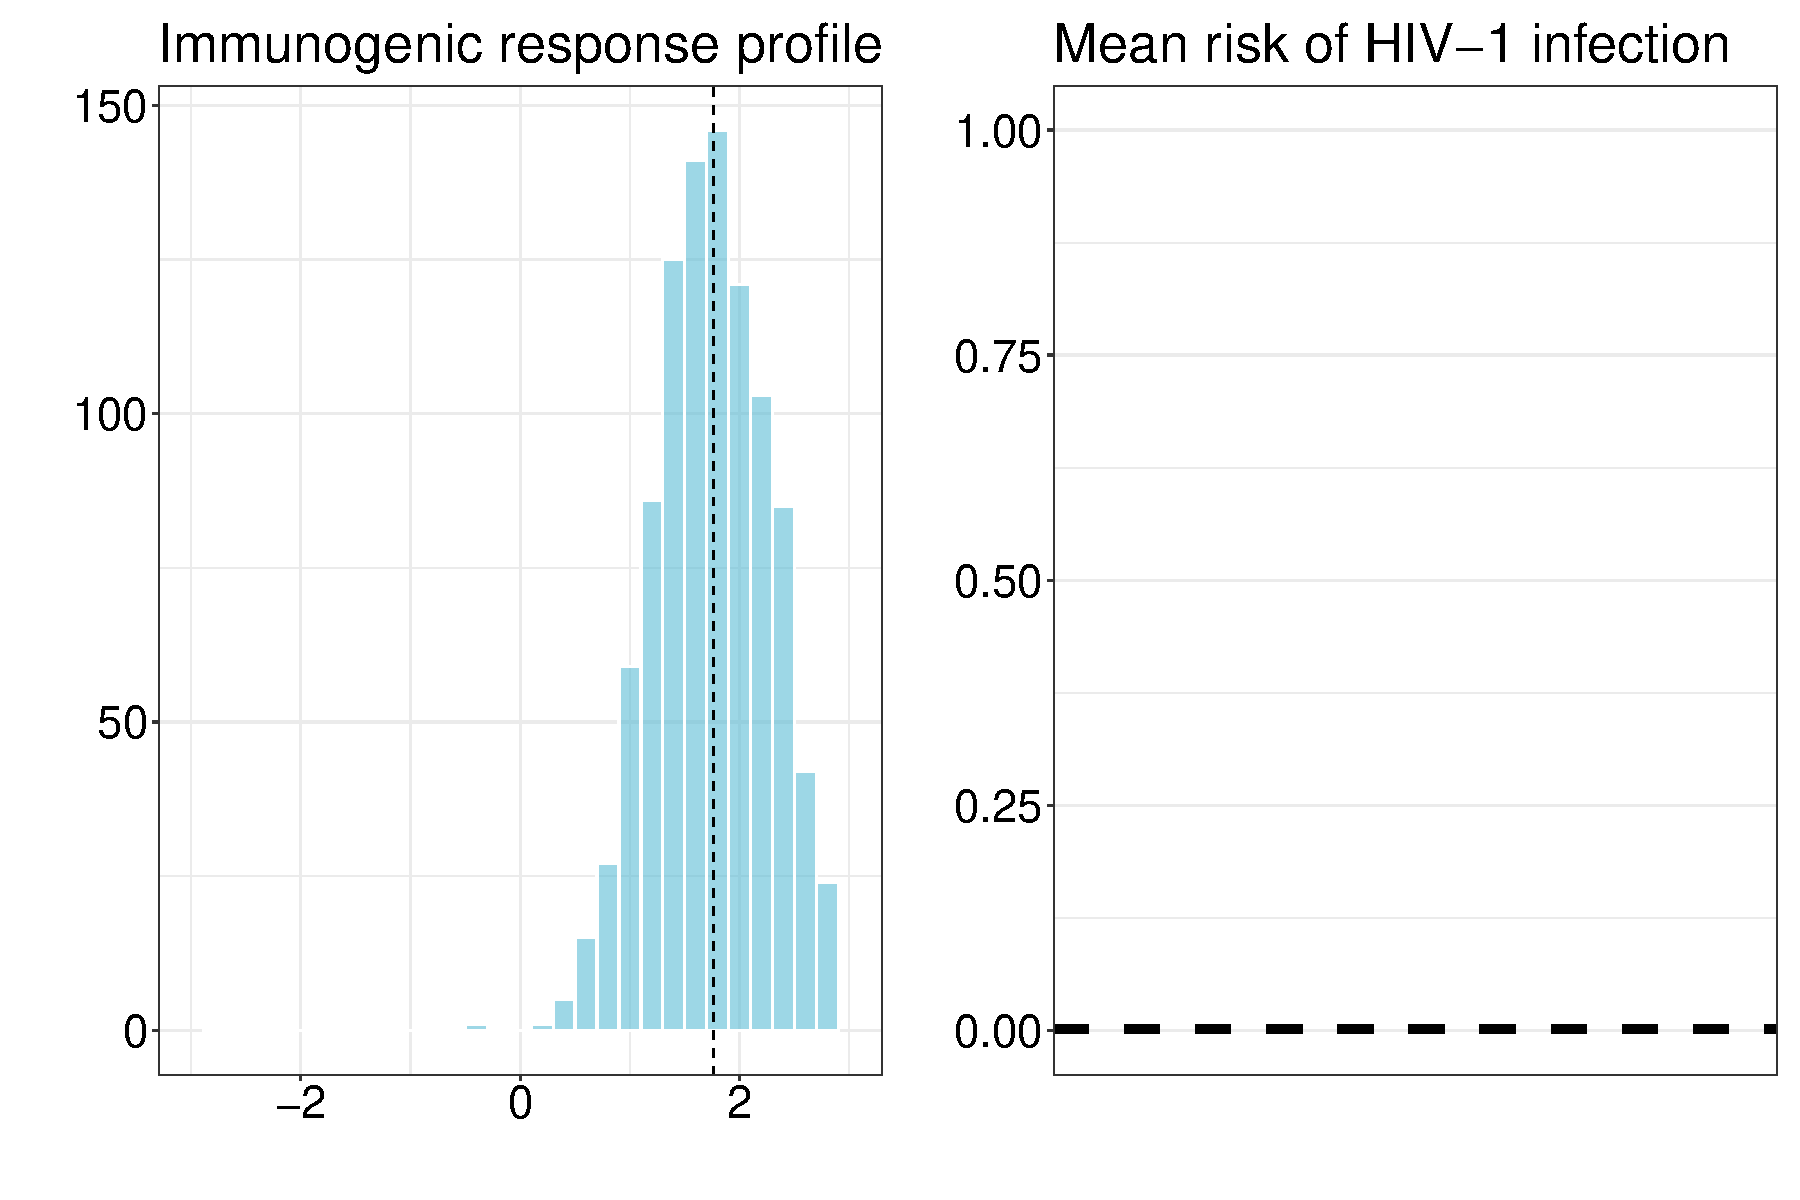
\includegraphics[scale=0.4]{shift-9}

\note{
}

\end{frame}

%%%%%%%%%%%%%%%%%%%%%%%%%%%%%%%%%%%%%%%%%%%%%%%%%%%%%%%%%%%%%%%%%%%%%%%%%%%%%%%%

\begin{frame}[c,noframenumbering]{HIV-1 risk under shifted immunogenic responses}

%\centering
\hspace*{-1cm}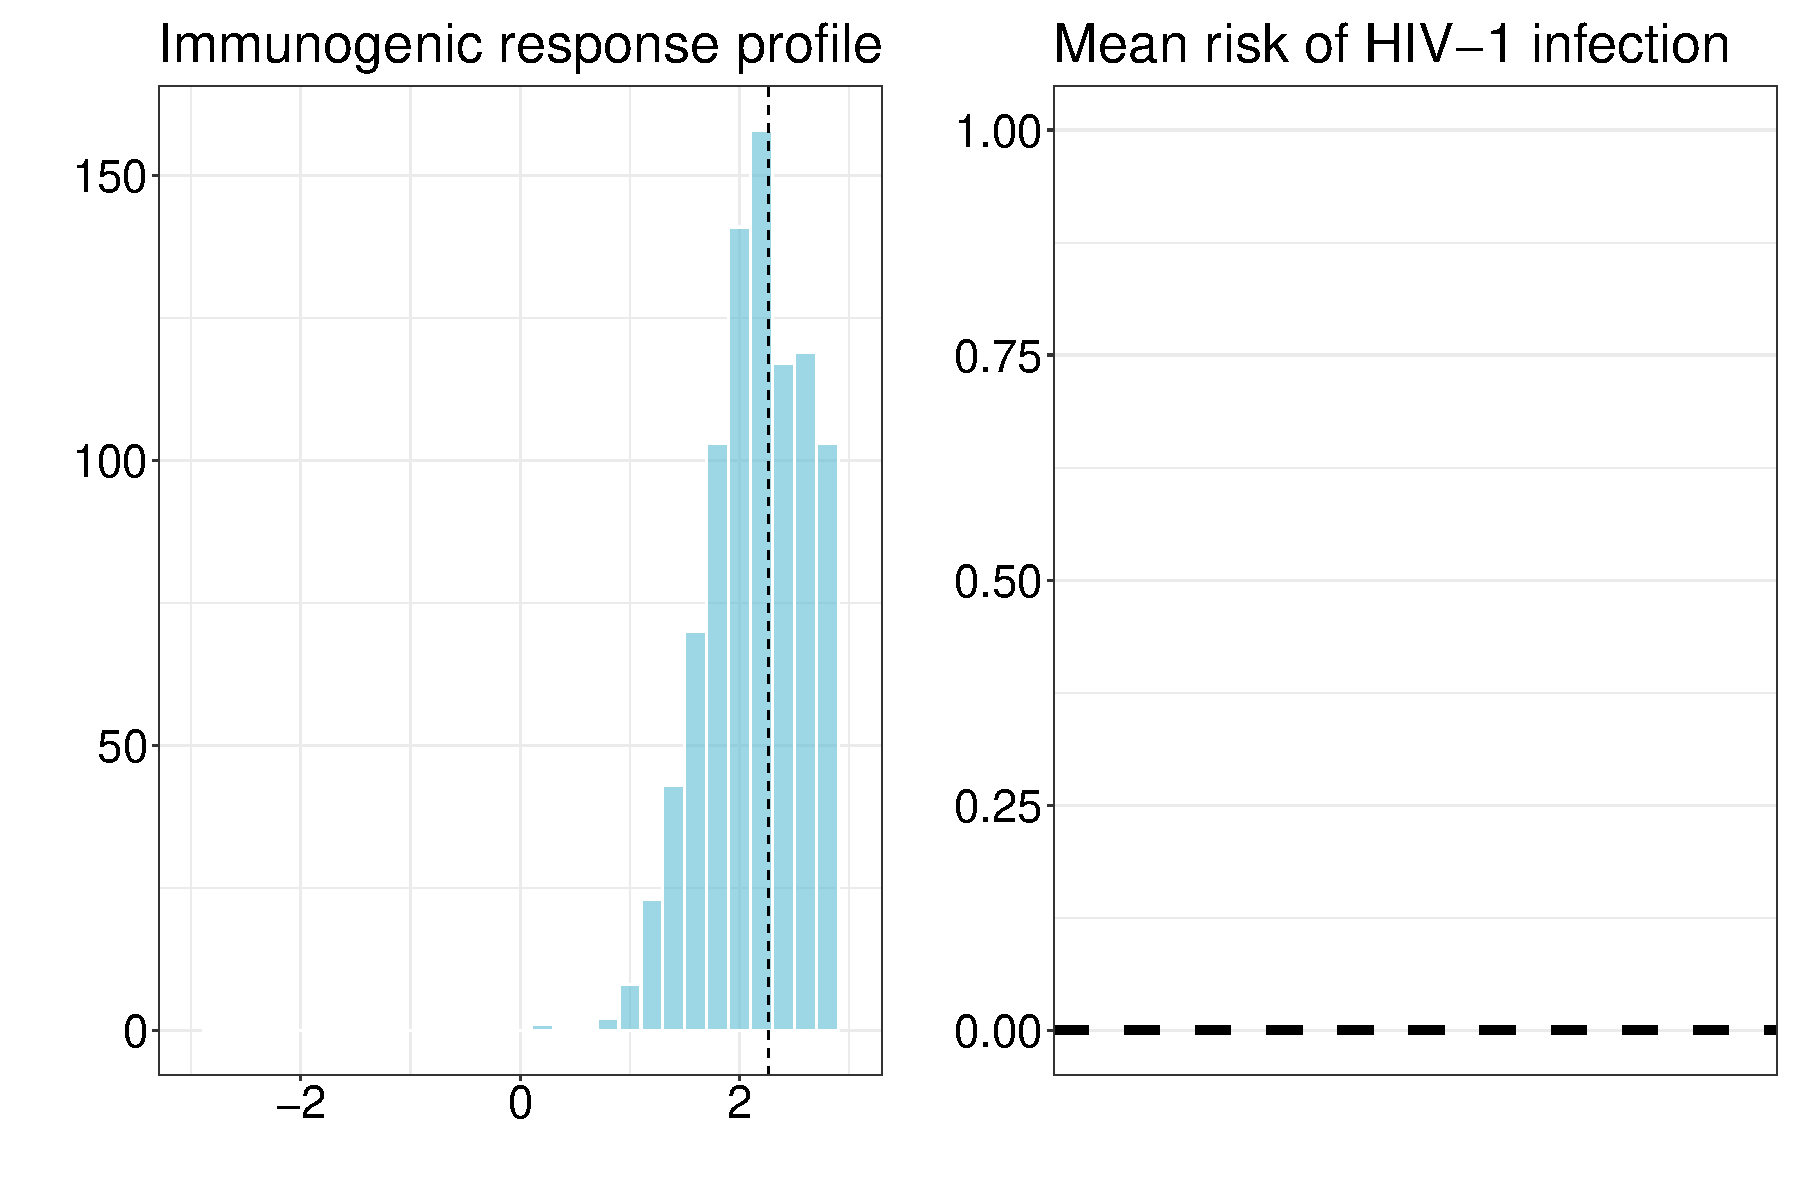
\includegraphics[scale=0.4]{shift-10}

\note{
}

\end{frame}

%%%%%%%%%%%%%%%%%%%%%%%%%%%%%%%%%%%%%%%%%%%%%%%%%%%%%%%%%%%%%%%%%%%%%%%%%%%%%%%%

\begin{frame}[c]{Efficient estimators in spite of two-phase sampling}

\begin{center}
\begin{itemize}
  \itemsep10pt
  \item What if sampling mechanism $\pi_0(Y, L) = \pr(C = 1 \mid Y, L)$
    is not known by design? Nonparametric estimation of $\pi_0(Y, L)$?
  \item Building on \cite{rose2011targeted2sd}, we provide
    \begin{itemize}
      \itemsep4pt
      \item asymptotically linear and nonparametric-\textit{efficient}
        estimators;
      \item multiply \textit{robust}, with \underline{two forms} of double
        robustness;
      \item Gaussian limit distributions and Wald-type confidence intervals.
    \end {itemize}
  \item New open source software for easily using these estimators:
    \begin{itemize}
      \itemsep4pt
      \item \url{https://github.com/nhejazi/haldensify} (densities)
      \item \url{https://github.com/nhejazi/txshift} (one-step, TMLE)
    \end {itemize}
\end{itemize}
\end{center}

\note{
\begin{itemize}
  \itemsep10pt
  \item \textbf{Asymptotic linearity:}
    \begin{equation*}
      \Psi(P_n^{\star}) - \Psi(P_0^X) = \frac{1}{n} \sum_{i = 1}^{n}
      D(P_0^X)(X_i) + o_P\left(\frac{1}{\sqrt{n}}\right)
    \end{equation*}
  \item \textbf{Gaussian limiting distribution:}
    \begin{equation*}
      \sqrt{n}(\Psi(P_n^{\star}) - \Psi(P_0^X)) \to N(0, Var(D(P_0^X)(X)))
    \end{equation*}
  \item \textbf{Statistical inference:}
    \begin{equation*}
      \text{Wald-type confidence interval}:
      \Psi(P_n^{\star}) \pm z_{\alpha} \cdot \frac{\sigma_n}{\sqrt{n}},
    \end{equation*}
    where $\sigma_n^2$ is computed directly via
    $\sigma_n^2 = \frac{1}{n} \sum_{i = 1}^{n} D^2(\cdot)(X_i)$.
\end{itemize}
}

\end{frame}

%%%%%%%%%%%%%%%%%%%%%%%%%%%%%%%%%%%%%%%%%%%%%%%%%%%%%%%%%%%%%%%%%%%%%%%%%%%%%%%%

\begin{frame}[c]{Fighting the HIV-1 epidemic~\citep{hejazi2020efficient}}

%\vspace{-1.5em}
\begin{figure}[H]
  \centering
  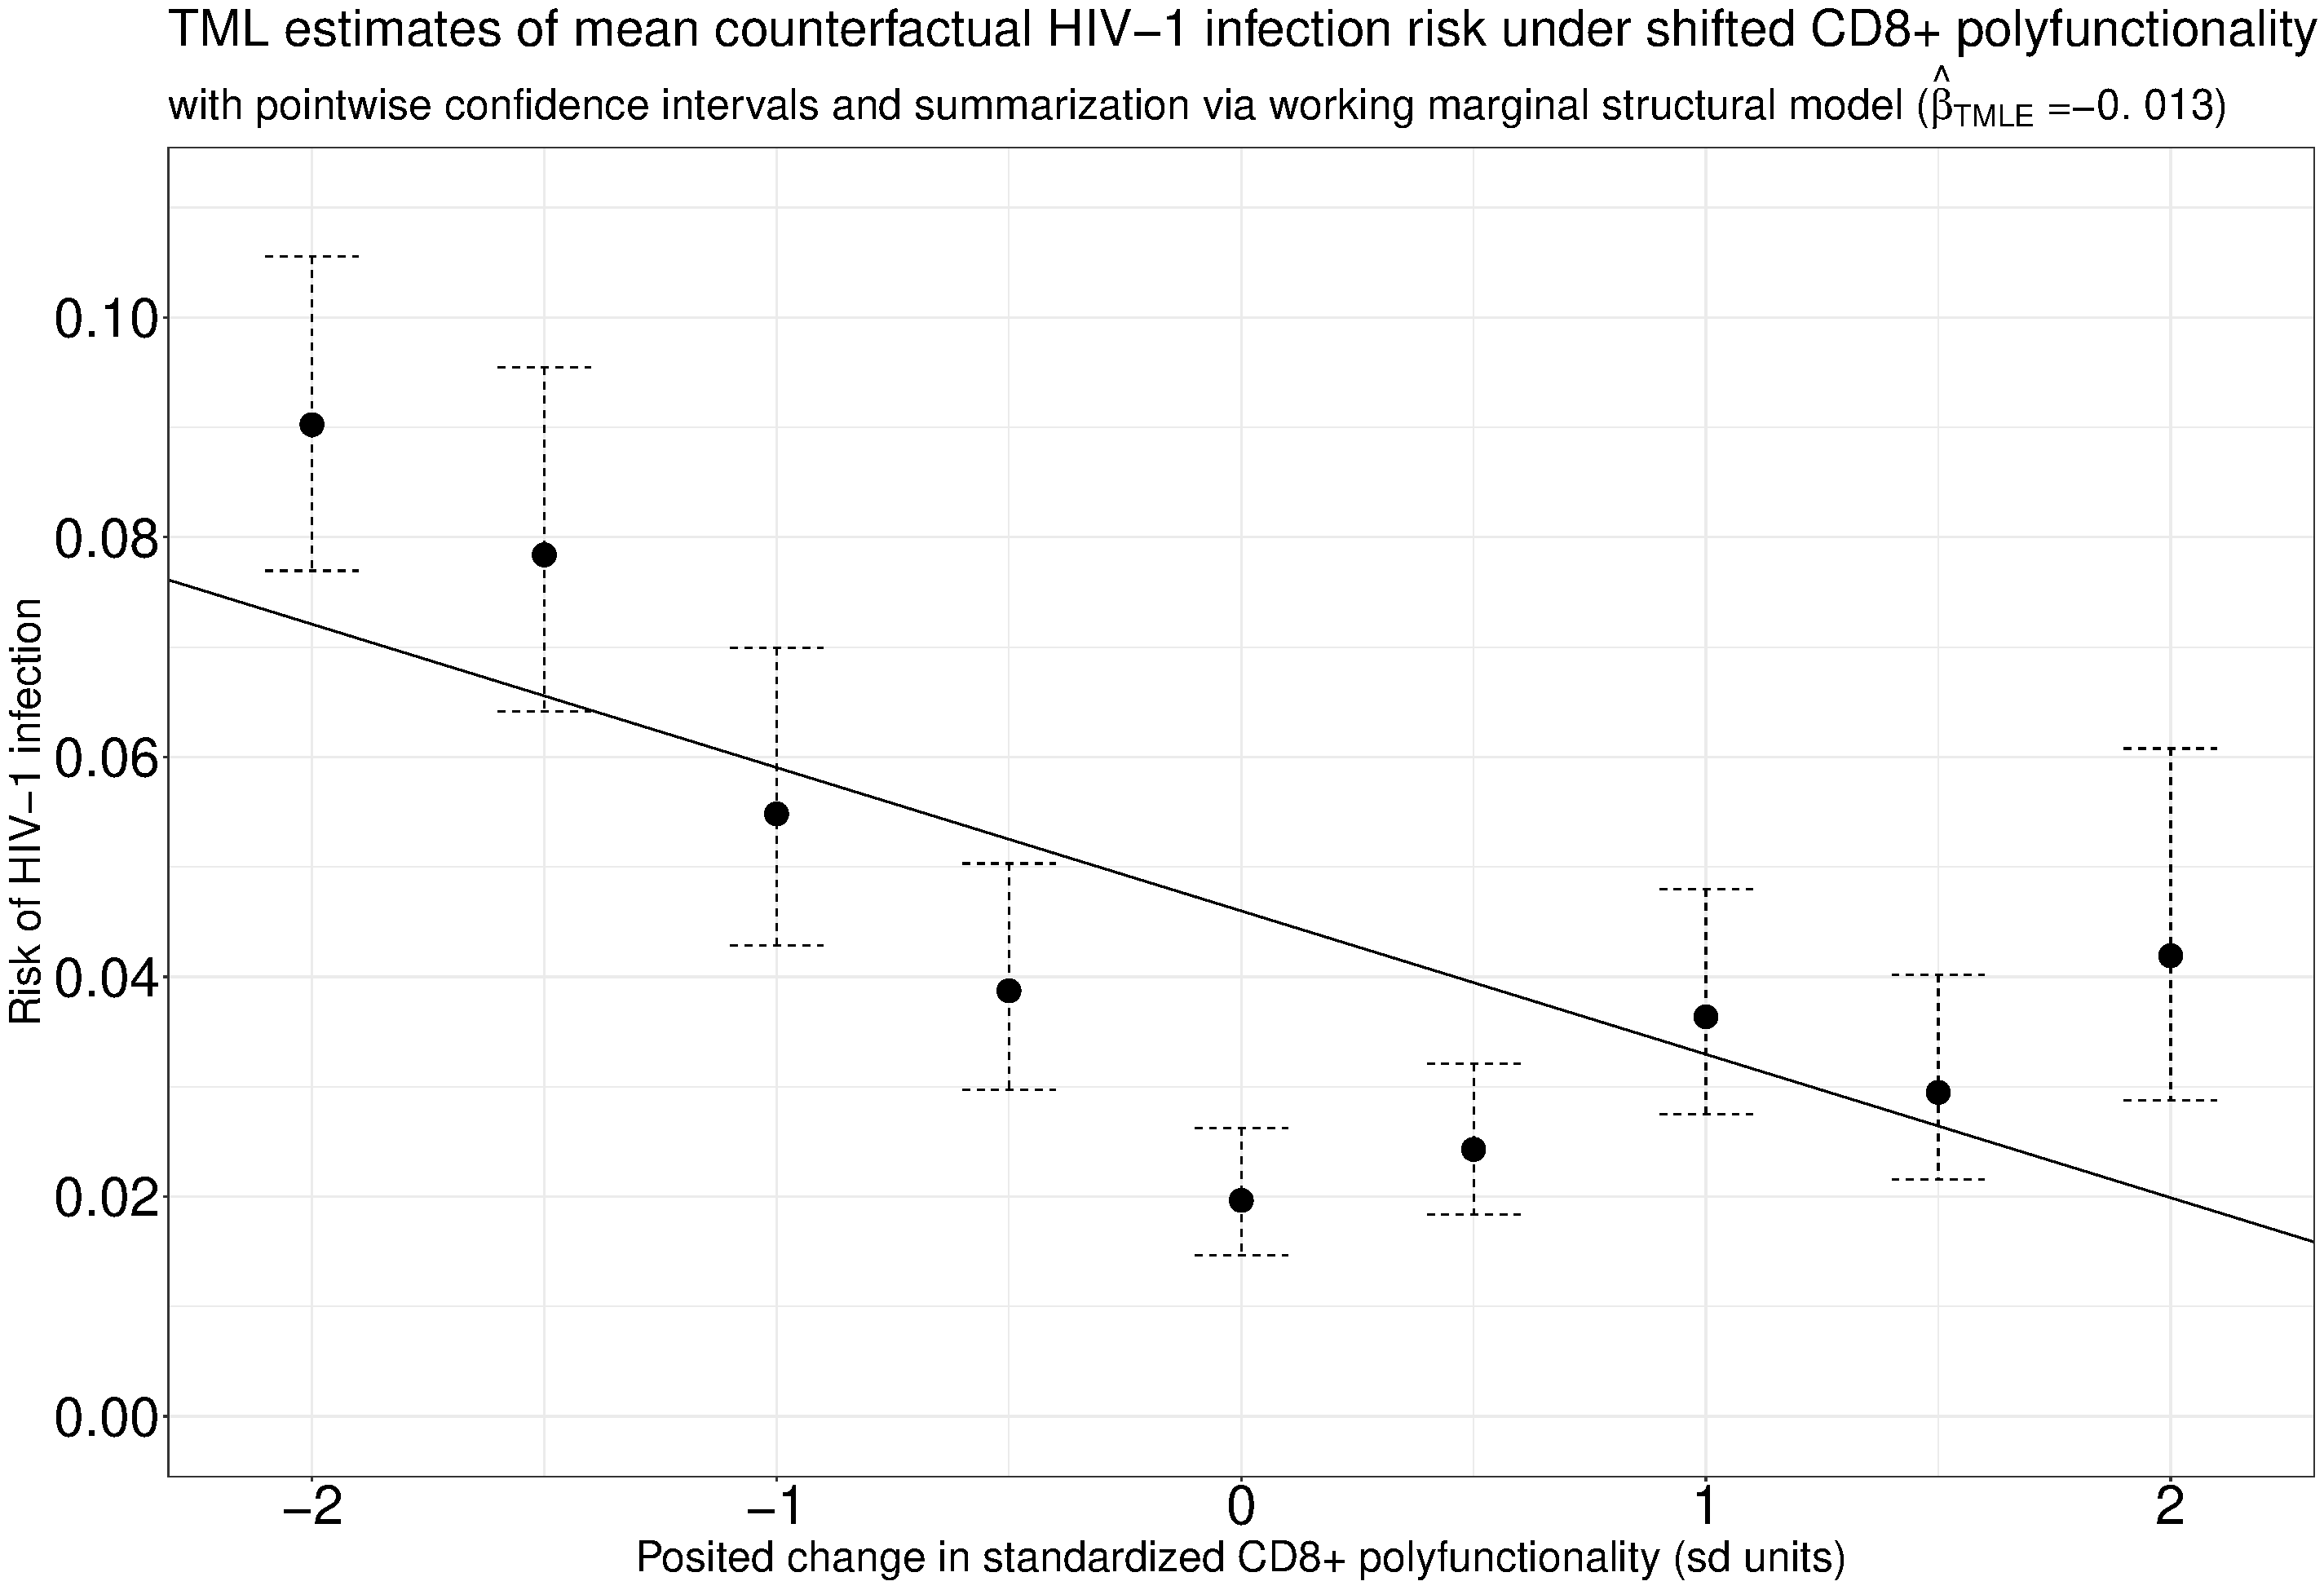
\includegraphics[scale=0.19]{cd8_msm_tmle_summary}
  \caption{
    Analysis of HIV-1 risk as a function of CD8+ immunogenicity, using
    \texttt{R} package \texttt{txshift}
    (\url{https://github.com/nhejazi/txshift}.)
  }
\end{figure}

\note{
}

\end{frame}

%%%%%%%%%%%%%%%%%%%%%%%%%%%%%%%%%%%%%%%%%%%%%%%%%%%%%%%%%%%%%%%%%%%%%%%%%%%%%%%%

\begin{frame}[c]{The big picture}

\begin{center}
\begin{itemize}
  \itemsep8pt
  %\item Vaccine efficacy evaluation helps to develop enhanced vaccines better
    %informed by biological properties of the target disease.
  \item We can target immunogenic responses modulated by HIV-1 vaccines to
    improve future efficacy against HIV-1.
  \item \textit{Stochastic} interventions constitute a flexible framework for
    considering \textbf{realistic} intervention policies.
  \item Large-scale vaccine trials often use two-phase designs --- need to
    (carefully!) adjust for sampling complications.
  \item We've developed open source software for assessing the causal effects
     of stochastic interventions in two-phase designs.
\end{itemize}
\end{center}

\note{
}

\end{frame}

%%%%%%%%%%%%%%%%%%%%%%%%%%%%%%%%%%%%%%%%%%%%%%%%%%%%%%%%%%%%%%%%%%%%%%%%%%%%%%%%

\begin{frame}[c]{Thank you!}

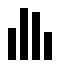
\includegraphics[scale=0.14]{homepage.png} \url{https://nimahejazi.org}

\vspace{2mm}

\includegraphics[scale=0.14]{twitter-icon.png}
  \url{https://twitter.com/nshejazi}

\vspace{2mm}
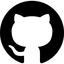
\includegraphics[scale=0.11]{github-icon.png}
  \url{https://github.com/nhejazi}

\vspace{2mm}

\includegraphics[scale=0.14]{paper-icon.png}
  \url{https://doi.org/10.1111/biom.13375}

\end{frame}

%%%%%%%%%%%%%%%%%%%%%%%%%%%%%%%%%%%%%%%%%%%%%%%%%%%%%%%%%%%%%%%%%%%%%%%%%%%%%%%%

\appendix
\begin{frame}[standout]
  Appendix
\end{frame}

%%%%%%%%%%%%%%%%%%%%%%%%%%%%%%%%%%%%%%%%%%%%%%%%%%%%%%%%%%%%%%%%%%%%%%%%%%%%%%%%

\begin{frame}[c]{From the causal to the statistical target parameter}

\begin{center}
\begin{tcolorbox}
\begin{assumption}{1}{\textit{Consistency}}\label{consistency}
  $Y^{d(a_i, l_i)}_i = Y_i$ in the event $A_i = d(a_i, l_i)$, for
  $i = 1, \ldots, n$
\end{assumption}
\end{tcolorbox}

\begin{tcolorbox}
\begin{assumption}{2}{\textit{SUTVA}}\label{sutva}
  $Y^{d(a_i, l_i)}_i$ does not depend on $d(a_j, l_j)$ for $i = 1,
  \ldots, n$ and $j \neq i$, or lack of interference
  \citep{rubin1978bayesian, rubin1980randomization}
\end{assumption}
\end{tcolorbox}

\begin{tcolorbox}
\begin{assumption}{3}{\textit{Strong ignorability}}\label{ignorability}
  $A_i \indep Y^{d(a_i, l_i)}_i \mid L_i$, for $i = 1, \ldots, n$
\end{assumption}
\end{tcolorbox}
\end{center}

\note{
}

\end{frame}

%%%%%%%%%%%%%%%%%%%%%%%%%%%%%%%%%%%%%%%%%%%%%%%%%%%%%%%%%%%%%%%%%%%%%%%%%%%%%%%%

\begin{frame}[c]{From the causal to the statistical target parameter}

\begin{center}
\begin{tcolorbox}
\begin{assumption}{4}{\textit{Positivity (or overlap)}}\label{positivity}
  $a_i \in \mathcal{A} \implies d(a_i, l_i) \in \mathcal{A}$ for all
  $l \in \mathcal{L}$, where $\mathcal{A}$ denotes the support of $A$
  conditional on $L = l_i$ for all $i = 1, \ldots n$
\end{assumption}
\end{tcolorbox}

\begin{itemize}
  \itemsep4pt
  \item This positivity assumption is not quite the same as that required for
    categorical interventions.
  \item In particular, we do not require that the intervention density place
    mass across all strata defined by $L$.
  \item Rather, we merely require the post-intervention quantity be seen in the
    observed data for given $a_i \in \mathcal{A}$ and $l_i \in \mathcal{L}$.
\end{itemize}
\end{center}

\note{
}

\end{frame}

%%%%%%%%%%%%%%%%%%%%%%%%%%%%%%%%%%%%%%%%%%%%%%%%%%%%%%%%%%%%%%%%%%%%%%%%%%%%%%%%

\begin{frame}[c]{NPSEM with static interventions}

\begin{center}
\begin{itemize}
  \itemsep10pt
  \item Use a nonparametric structural equation model (NPSEM) to describe the
    generation of $X$ \citep{pearl2009causality}, specifically
    \begin{equation*}
      L = f_L(U_L); A = f_A(L, U_A); Y = f_Y(A, L, U_Y)
    \end{equation*}
  \item Implies a model for the distribution of counterfactual random variables
    generated by interventions on the process.
  \item A \textit{static intervention} replaces $f_A$ with a specific value $a$
    in its conditional support $A \mid L$.
  \item This requires specifying a particular value of the exposure under which
    to evaluate the outcome \textit{a priori}.
\end{itemize}
\end{center}

\note{
}

\end{frame}

%%%%%%%%%%%%%%%%%%%%%%%%%%%%%%%%%%%%%%%%%%%%%%%%%%%%%%%%%%%%%%%%%%%%%%%%%%%%%%%%

\begin{frame}[c]{NPSEM with stochastic interventions}

\begin{center}
\begin{itemize}
  \itemsep10pt
  \item \textit{Stochastic interventions} modify the value $A$ would naturally
    assume by drawing from a modified exposure distribution.
  \item Consider the post-intervention value $A^{\star} \sim G^{\star}(\cdot
    \mid L)$; static interventions are a special case (degenerate distribution).
  \item Such an intervention generates a counterfactual random variable
    $Y_{G^{\star}} \coloneqq f_Y(A^{\star}, L, U_Y)$, with distribution
    $P_0^{\delta}$, .
  \item We aim to estimate $\psi_{0,\delta} \coloneqq \E_{P_0^{\delta}}
    \{Y_{G^{\star}}\}$, the counterfactual mean under the post-intervention
    exposure distribution $G^{\star}$.
\end{itemize}
\end{center}

\note{
}

\end{frame}

%%%%%%%%%%%%%%%%%%%%%%%%%%%%%%%%%%%%%%%%%%%%%%%%%%%%%%%%%%%%%%%%%%%%%%%%%%%%%%%%

\begin{frame}[c]{Stochastic interventions for the causal effects of shifts}

\begin{center}
\begin{itemize}
  \itemsep10pt
  \item \cite{diaz2012population, diaz2018stochastic}'s \textit{stochastic}
    interventions
     \begin{equation*}\label{shift_intervention}
       d(a, l) =
         \begin{cases}
           a + \delta, & a + \delta < u(l) \quad (\text{if plausible}) \\
           a, & a + \delta \geq u(l) \quad (\text{otherwise})
         \end{cases}
     \end{equation*}
  \item Our estimand is $\psi_{0, d} \coloneqq \E_{P_0^d}\{Y_{d(A,L)}\}$, mean
    of $Y_{d(A, L)}$.
  \item Statistical target parameter is
    $\Psi(P_0^X) = \E_{P_0^X}{\overline{Q}(d(A, L), L)}$, counterfactual mean
    of the \textit{shifted} outcome mechanism.
  \item For HVTN 505, $\psi_{0,d}$ is the counterfactual risk of HIV-1
    infection, had the observed value of the immune response been altered under
    the rule $d(A,L)$ defining $G^{\star}(\cdot \mid L)$.
\end{itemize}
\end{center}

\note{
  \begin{itemize}
  \item Causal estimand: counterfactual mean of HIV-1 infection (risk) under a
    \textit{shifted} immunogenic response distribution.
  \end{itemize}
}

\end{frame}

%%%%%%%%%%%%%%%%%%%%%%%%%%%%%%%%%%%%%%%%%%%%%%%%%%%%%%%%%%%%%%%%%%%%%%%%%%%%%%%%

\begin{frame}[c]{Literature: \cite{diaz2012population}}

\begin{center}
\begin{itemize}
  \itemsep10pt
  \item \textit{Proposal:} Evaluate outcome under an altered
    \textit{intervention distribution} --- e.g.,
    $P_{\delta}(g_0)(A = a \mid L) = g_0(a - \delta(L) \mid L)$.
  \item Identification conditions for a statistical parameter of the
    counterfactual outcome $\psi_{0,d}$ under such an intervention.
  \item Show that the causal quantity of interest $\E_0 \{Y_{d(A, L)}\}$ is
    identified by a functional of the distribution of $X$:
    \begin{align*}\label{eqn:identification2012}
      \psi_{0,d} = \int_{\mathcal{L}} \int_{\mathcal{A}} &\E_{P_0^X} \{Y \mid
        A = d(a, l), L = l\} \cdot \\ &q_{0, A}^X(a \mid L = l) \cdot
        q_{0, L}^X(l) d\mu(a)d\nu(l)
    \end{align*}
  \item Provides a derivation based on the efficient influence function (EIF)
    with respect to the nonparametric model $\mathcal{M}$.
\end{itemize}
\end{center}

\note{
  \begin{itemize}
    \item The identification result allows us to write down the causal quantity
      of interest in terms of a functional of the observed data.
    \item Key innovation: loosening standard assumptions through a change in
      the observed intervention mechanism.
    \item Problem: globally altering an intervention mechanism does not
      necessarily respect individual characteristics.
    \item The authors build IPW, A-IPW, and TML estimators, comparing the three
      different approaches.
    \item IMPORTANT: gives the g-computation formula for identification of this
      estimator from the observed data structure.
  \end{itemize}
}

\end{frame}

%%%%%%%%%%%%%%%%%%%%%%%%%%%%%%%%%%%%%%%%%%%%%%%%%%%%%%%%%%%%%%%%%%%%%%%%%%%%%%%%

\begin{frame}[c]{Literature: \cite{haneuse2013estimation}}

\begin{center}
\begin{itemize}
  \itemsep10pt
  \item \textit{Proposal:} Characterization of stochastic interventions as
    \textit{modified treatment policies} (MTPs).
  \item Assumption of \textit{piecewise smooth invertibility} allows for the
    intervention distribution of any MTP to be recovered:
    \begin{equation*}
      g_{0, \delta}(a \mid l) = \sum_{j = 1}^{J(l)} I_{\delta, j} \{h_j(a, l),
      l\} g_0\{h_j(a, l) \mid l\} h^{'}_j(a,l)
    \end{equation*}
  \item Such intervention policies account for the natural value of the
    intervention $A$ directly yet are interpretable as the imposition of an
    altered intervention mechanism.
  \item Identification conditions for assessing the parameter of interest under
    such interventions appear technically complex (at first).
\end{itemize}
\end{center}

\note{
  \begin{itemize}
    \item Shifts of the form $d(A,L)$ are considerably more interesting since
      these are realistic intervention policies.
    \item Example: consider an individual with an extremely high immune response
      but whose baseline covariates $L$ suggest we shift the response still
      higher. Such a shift may not be biologically plausible (impossible, even)
      but we cannot account for this if the shift is only a function of $L$.
    \item The authors build IPW, outcome regression, and non-iterative doubly
      robust estimators, as well as an approach based on MSMs.
    \item Piecewise smooth invertibility: This assumption ensures that we can
      use the change of variable formula when computing integrals over $A$ and
      it is useful to study the estimators that we propose in this paper.
  \end{itemize}
}

\end{frame}

%%%%%%%%%%%%%%%%%%%%%%%%%%%%%%%%%%%%%%%%%%%%%%%%%%%%%%%%%%%%%%%%%%%%%%%%%%%%%%%%

\begin{frame}[c]{Literature: \cite{young2014identification}}

\begin{center}
\begin{itemize}
  \itemsep10pt
  \item Establishes equivalence between g-formula when proposed intervention
    depends on natural value and when it does not.
  \item This equivalence leads to a sufficient positivity condition for
    estimating the counterfactual mean under MTPs via the same statistical
    functional studied in \cite{diaz2012population}.
  \item Extends earlier identification results, providing a way to use the same
    statistical functional to assess $\E Y_{d(A,L)}$ or $\E Y_{d(L)}$.
  \item The authors also consider limits on implementing shifts $d(A,L)$, and
    address working in a longitudinal setting.
\end{itemize}
\end{center}

\note{
}

\end{frame}

%%%%%%%%%%%%%%%%%%%%%%%%%%%%%%%%%%%%%%%%%%%%%%%%%%%%%%%%%%%%%%%%%%%%%%%%%%%%%%%%

\begin{frame}[c]{Literature: \cite{diaz2018stochastic}}

\begin{center}
\begin{itemize}
  \itemsep10pt
  \item Builds on the original proposal, accomodating MTP-type shifts $d(A,L)$
    proposed after their earlier work.
  \item To protect against positivity violations, considers a specific shifting
    mechanism:
     \begin{equation*}\label{shift_intervention}
       d(a, l) =
         \begin{cases}
           a + \delta, & a + \delta < u(l) \\
           a, & \text{otherwise}
         \end{cases}
     \end{equation*}
  \item Proposes an improved ``1-TMLE'' algorithm, with a single auxiliary
    covariate for constructing the TML estimator.
  \item Our (first) contribution: implementation of this algorithm.
\end{itemize}
\end{center}

\note{
}

\end{frame}

%%%%%%%%%%%%%%%%%%%%%%%%%%%%%%%%%%%%%%%%%%%%%%%%%%%%%%%%%%%%%%%%%%%%%%%%%%%%%%%%

\begin{frame}[c]{Flexible, efficient estimation}

\begin{center}
\begin{itemize}
  \itemsep10pt
  \item The efficient influence function (EIF) is:
    \begin{equation*}
      D(P_0^X)(x) = H(a, l)({y - \overline{Q}(a, l)}) +
      \overline{Q}(d(a, l), l) - \Psi(P_0^X).
    \end{equation*}
  \item The one-step estimator corrects bias by adding the empirical mean of the
    estimated EIF to the substitution estimator:
    \begin{equation*}\label{tmle}
        \Psi_n^{+} = \frac{1}{n} \sum_{i = 1}^n \overline{Q}_n(d(A_i, L_i),
        L_i) + D_n(O_i).
      \end{equation*}
  \item The TML estimator is built by updating initial estimates of
    $\overline{Q}_n$ via a (logistic) tilting model, yielding
    \begin{equation*}\label{tmle}
      \Psi_n^{\star} = \frac{1}{n} \sum_{i = 1}^n
      \overline{Q}_n^{\star}(d(A_i, L_i), L_i).
      \end{equation*}
  \item Both estimators are CAN even when nuisance parameters are estimated via
    flexible, machine learning techniques.
\end{itemize}
\end{center}

\note{
  \begin{itemize}
    \item Semiparametric-efficient estimation thru solving efficient influence
      function estimating equation wrt the model $\M$.
    \item The auxiliary covariate simplifies when the treatment is in the limits
      (conditional on $W$) --- i.e., for $A_i \in (u(l) - \delta, u(l))$, then
      we have $H(a,l) = \frac{g_0(a - \delta \mid l)}{g_0(a \mid l)} + 1$.
    \item Need to explicitly remind the audience what $u(l)$ is again. It's only
      appeared once at this point, and only been mentioned in passing.
  \end{itemize}
}

\end{frame}

%%%%%%%%%%%%%%%%%%%%%%%%%%%%%%%%%%%%%%%%%%%%%%%%%%%%%%%%%%%%%%%%%%%%%%%%%%%%%%%%

\begin{frame}[c]{Augmented estimators for two-phase sampling designs}

\begin{center}
\begin{itemize}
  \itemsep10pt
  \item \cite{rose2011targeted2sd} introduce the IPCW-TMLE, to be used when
    observed data is subject to two-phase sampling.
  \item \textit{Initial proposal:} correct for two-phase sampling by using a
    loss function with inverse probability of censoring weights:
    \begin{equation*}
      \lik(P_0^X)(O) = \frac{C}{\pi_0(Y, L)}\lik^F(P_0^X)(X)
    \end{equation*}
  \item When the sampling mechanism $\pi_0(Y,L)$ can be estimated by
    a parametric form, this procedure yields an efficient estimator.
  \item However, when machine learning is used (e.g., when $\pi_0(Y,L)$ is not
    \textit{known by design}), this is insufficient.
\end{itemize}
\end{center}

\note{
}

\end{frame}

%%%%%%%%%%%%%%%%%%%%%%%%%%%%%%%%%%%%%%%%%%%%%%%%%%%%%%%%%%%%%%%%%%%%%%%%%%%%%%%%

\begin{frame}[c]{Efficient estimation and multiple robustness}

\begin{center}
\begin{itemize}
  \itemsep10pt
  \item Then, the IPCW augmentation must be applied to the EIF:
    \begin{align*}
      D(P_0^X)(o) = &\frac{c}{\pi_0(y, l)} D^F(P_0^X)(x) - \left(1 -
        \frac{c}{\pi_0(y, l)}\right) \cdot \\ &\E(D^F(P_0^X)(x) \mid
        C = 1, Y = y, L = l),
    \end{align*}
   \begin{itemize}
    \itemsep6pt
     \item Expresses observed data EIF $D^F(P_0^X)(o)$ in terms of full data
       EIF $D^F(P_0^X)(x)$; inclusion of second term ensures efficiency.
     \item The expectation of the full data EIF $D^F(P_0^X)(x)$, taken only over
      units selected by the sampling mechanism (i.e., $C = 1$).
  \end{itemize}
 \item A unique multiple robustness property --- combinations of
    $(g_0(L), \overline{Q}_0(A,L)) \times (\pi_0(Y, L), \E(D^F(P^X_0)(x) \mid
    C = 1, Y, L))$.
\end{itemize}
\end{center}

\note{
}

\end{frame}

%%%%%%%%%%%%%%%%%%%%%%%%%%%%%%%%%%%%%%%%%%%%%%%%%%%%%%%%%%%%%%%%%%%%%%%%%%%%%%%%

%%%%%%%%%%%%%%%%%%%%%%%%%%%%%%%%%%%%%%%%%%%%%%%%%%%%%%%%%%%%%%%%%%%%%%%%%%%%%%%%

\begin{frame}[c]{Algorithm for TML estimation}

\begin{center}
\begin{enumerate}\label{tmle_algo}
  \itemsep6pt
  \item Construct initial estimators $g_n$ of $g_0(A, L)$ and $Q_n$ of
    $\overline{Q}_0(A, L)$, perhaps using data-adaptive regression techniques.
  \item For each observation $i$, compute an estimate $H_n(a_i, l_i)$ of the
    auxiliary covariate $H(a_i,l_i)$.
  \item Estimate the parameter $\epsilon$ in the logistic regression model
    $$\text{logit}\overline{Q}_{\epsilon, n}(a, l) =
    \text{logit}\overline{Q}_n(a, l) + \epsilon H_n(a, l),$$
    or an alternative regression model incorporating weights.
  \item Compute TML estimator $\Psi_n$ of the target parameter, defining update
    $\overline{Q}_n^{\star}$ of the initial estimate
    $\overline{Q}_{n, \epsilon_n}$:
    \begin{equation*}\label{tmle}
      \Psi_n = \Psi(P_n^{\star}) = \frac{1}{n} \sum_{i = 1}^n
        \overline{Q}_n^{\star}(d(A_i, L_i), L_i).
      \end{equation*}
\end{enumerate}
\end{center}

\note{
  \begin{itemize}
    \item We recommend using nonparametric methods for the initial estimators,
      as consistent estimation is necessary for efficiency of the estimator
      $\Psi_n$.
    \item Intuition for the submodel fluctuation?
  \end{itemize}
}

\end{frame}

%%%%%%%%%%%%%%%%%%%%%%%%%%%%%%%%%%%%%%%%%%%%%%%%%%%%%%%%%%%%%%%%%%%%%%%%%%%%%%%%

\begin{frame}[c]{Algorithm for IPCW-TML estimation}

\begin{center}
\begin{enumerate}\label{ipcwtmle_algo}
  \itemsep8pt
  \item Using all observed units ($X$), estimate sampling mechanism
    $\pi(Y, L)$, perhaps using data-adaptive regression methods.
  \item Using only observed units in the two-phase sample $C = 1$,
    construct initial estimators $g_n(A,L)$ and $\overline{Q}_n(A,L)$,
    weighting by the sampling mechanism estimate $\pi_n(Y,L)$.
  \item With the approach described for the full data case, compute
    $H_n(a_i,l_i)$, and fluctuate submodel via logistic regression.
  \item Compute IPCW-TML estimator $\Psi_n$ of the target parameter, by solving
    the IPCW-augmented EIF estimating equation.
  \item Iteratively update estimated sampling weights $\pi_n(Y,L)$ and
    IPCW-augmented EIF, updating TML estimate in each iteration, until
    $\frac{1}{n}\sum_{i = 1}^n \text{EIF}_i < \frac{1}{n}$.
\end{enumerate}
\end{center}

\note{
  \begin{itemize}
    \item We recommend using nonparametric methods for the initial estimators,
      as consistent estimation is necessary for efficiency of the estimator
      $\Psi_n$.
    \item Intuition for the submodel fluctuation?
    \item This process includes the use of HAL to fit the regression of the EIF
      contributions on the sampling node $\{Y, L\}$.
  \end{itemize}
}

\end{frame}

%%%%%%%%%%%%%%%%%%%%%%%%%%%%%%%%%%%%%%%%%%%%%%%%%%%%%%%%%%%%%%%%%%%%%%%%%%%%%%%%

\begin{frame}[c]{Key properties of TML estimators}

\begin{center}
\begin{itemize}
  \itemsep10pt
  \item \textbf{Asymptotic linearity:}
    \begin{equation*}
      \Psi(P_n^{\star}) - \Psi(P_0^X) = \frac{1}{n} \sum_{i = 1}^{n}
      D(P_0^X)(X_i) + o_P\left(\frac{1}{\sqrt{n}}\right)
    \end{equation*}
  \item \textbf{Gaussian limiting distribution:}
    \begin{equation*}
      \sqrt{n}(\Psi(P_n^{\star}) - \Psi(P_0^X)) \to N(0, Var(D(P_0^X)(X)))
    \end{equation*}
  \item \textbf{Statistical inference:}
    \begin{equation*}
      \text{Wald-type confidence interval}: \Psi(P_n^{\star}) \pm z_{1 -
      \frac{\alpha}{2}} \cdot \frac{\sigma_n}{\sqrt{n}},
    \end{equation*}
    where $\sigma_n^2$ is computed directly via
    $\sigma_n^2 = \frac{1}{n} \sum_{i = 1}^{n} D^2(\cdot)(X_i)$.
\end{itemize}
\end{center}

\note{
Under the additional condition that the remainder term $R(\hat{P}^{\star},
P_0)$ decays as $o_P \left( \frac{1}{\sqrt{n}} \right),$ we have that
$\Psi_n - \Psi_0 = (P_n - P_0) \cdot D(P_0) + o_P
\left( \frac{1}{\sqrt{n}} \right),$ which, by a central limit theorem,
establishes a Gaussian limiting distribution for the estimator, with variance
$V(D(P_0))$, the variance of the efficient influence function
when $\Psi$ admits an asymptotically linear representation.

The above implies that $\Psi_n$ is a $\sqrt{n}$-consistent estimator of $\Psi$,
that it is asymptotically normal (as given above), and that it is locally
efficient. This allows us to build Wald-type confidence intervals, where
$\sigma_n^2$ is an estimator of $V(D(P_0))$. The estimator $\sigma_n^2$
may be obtained using the bootstrap or computed directly via
$\sigma_n^2 = \frac{1}{n} \sum_{i = 1}^{n} D^2(\bar{Q}_n^{\star}, g_n)(O_i)$

We obtain semiparametric-efficient estimation and robust inference in the
nonparametric model $\M$ by solving the efficient influence function.

\begin{enumerate}
   \item If $D(\bar{Q}_n^*, g_n)$ converges to $D(P_0)$ in $L_2(P_0)$ norm.
   \item The size of the class of functions $\bar{Q}_n^{\star}$ and $g_n$ is
     bounded (technically, $\exists \mathcal{F}$ st
     $D(\bar{Q}_n^*, g_n) \in \mathcal{F}$ whp, where $\mathcal{F}$ is a
     Donsker class)
\end{enumerate}
}

\end{frame}

%%%%%%%%%%%%%%%%%%%%%%%%%%%%%%%%%%%%%%%%%%%%%%%%%%%%%%%%%%%%%%%%%%%%%%%%%%%%%%%%

\begin{frame}[c]{Identifying the best efficient estimator}

%\vspace{-1.5em}
\begin{figure}[H]
  \centering
  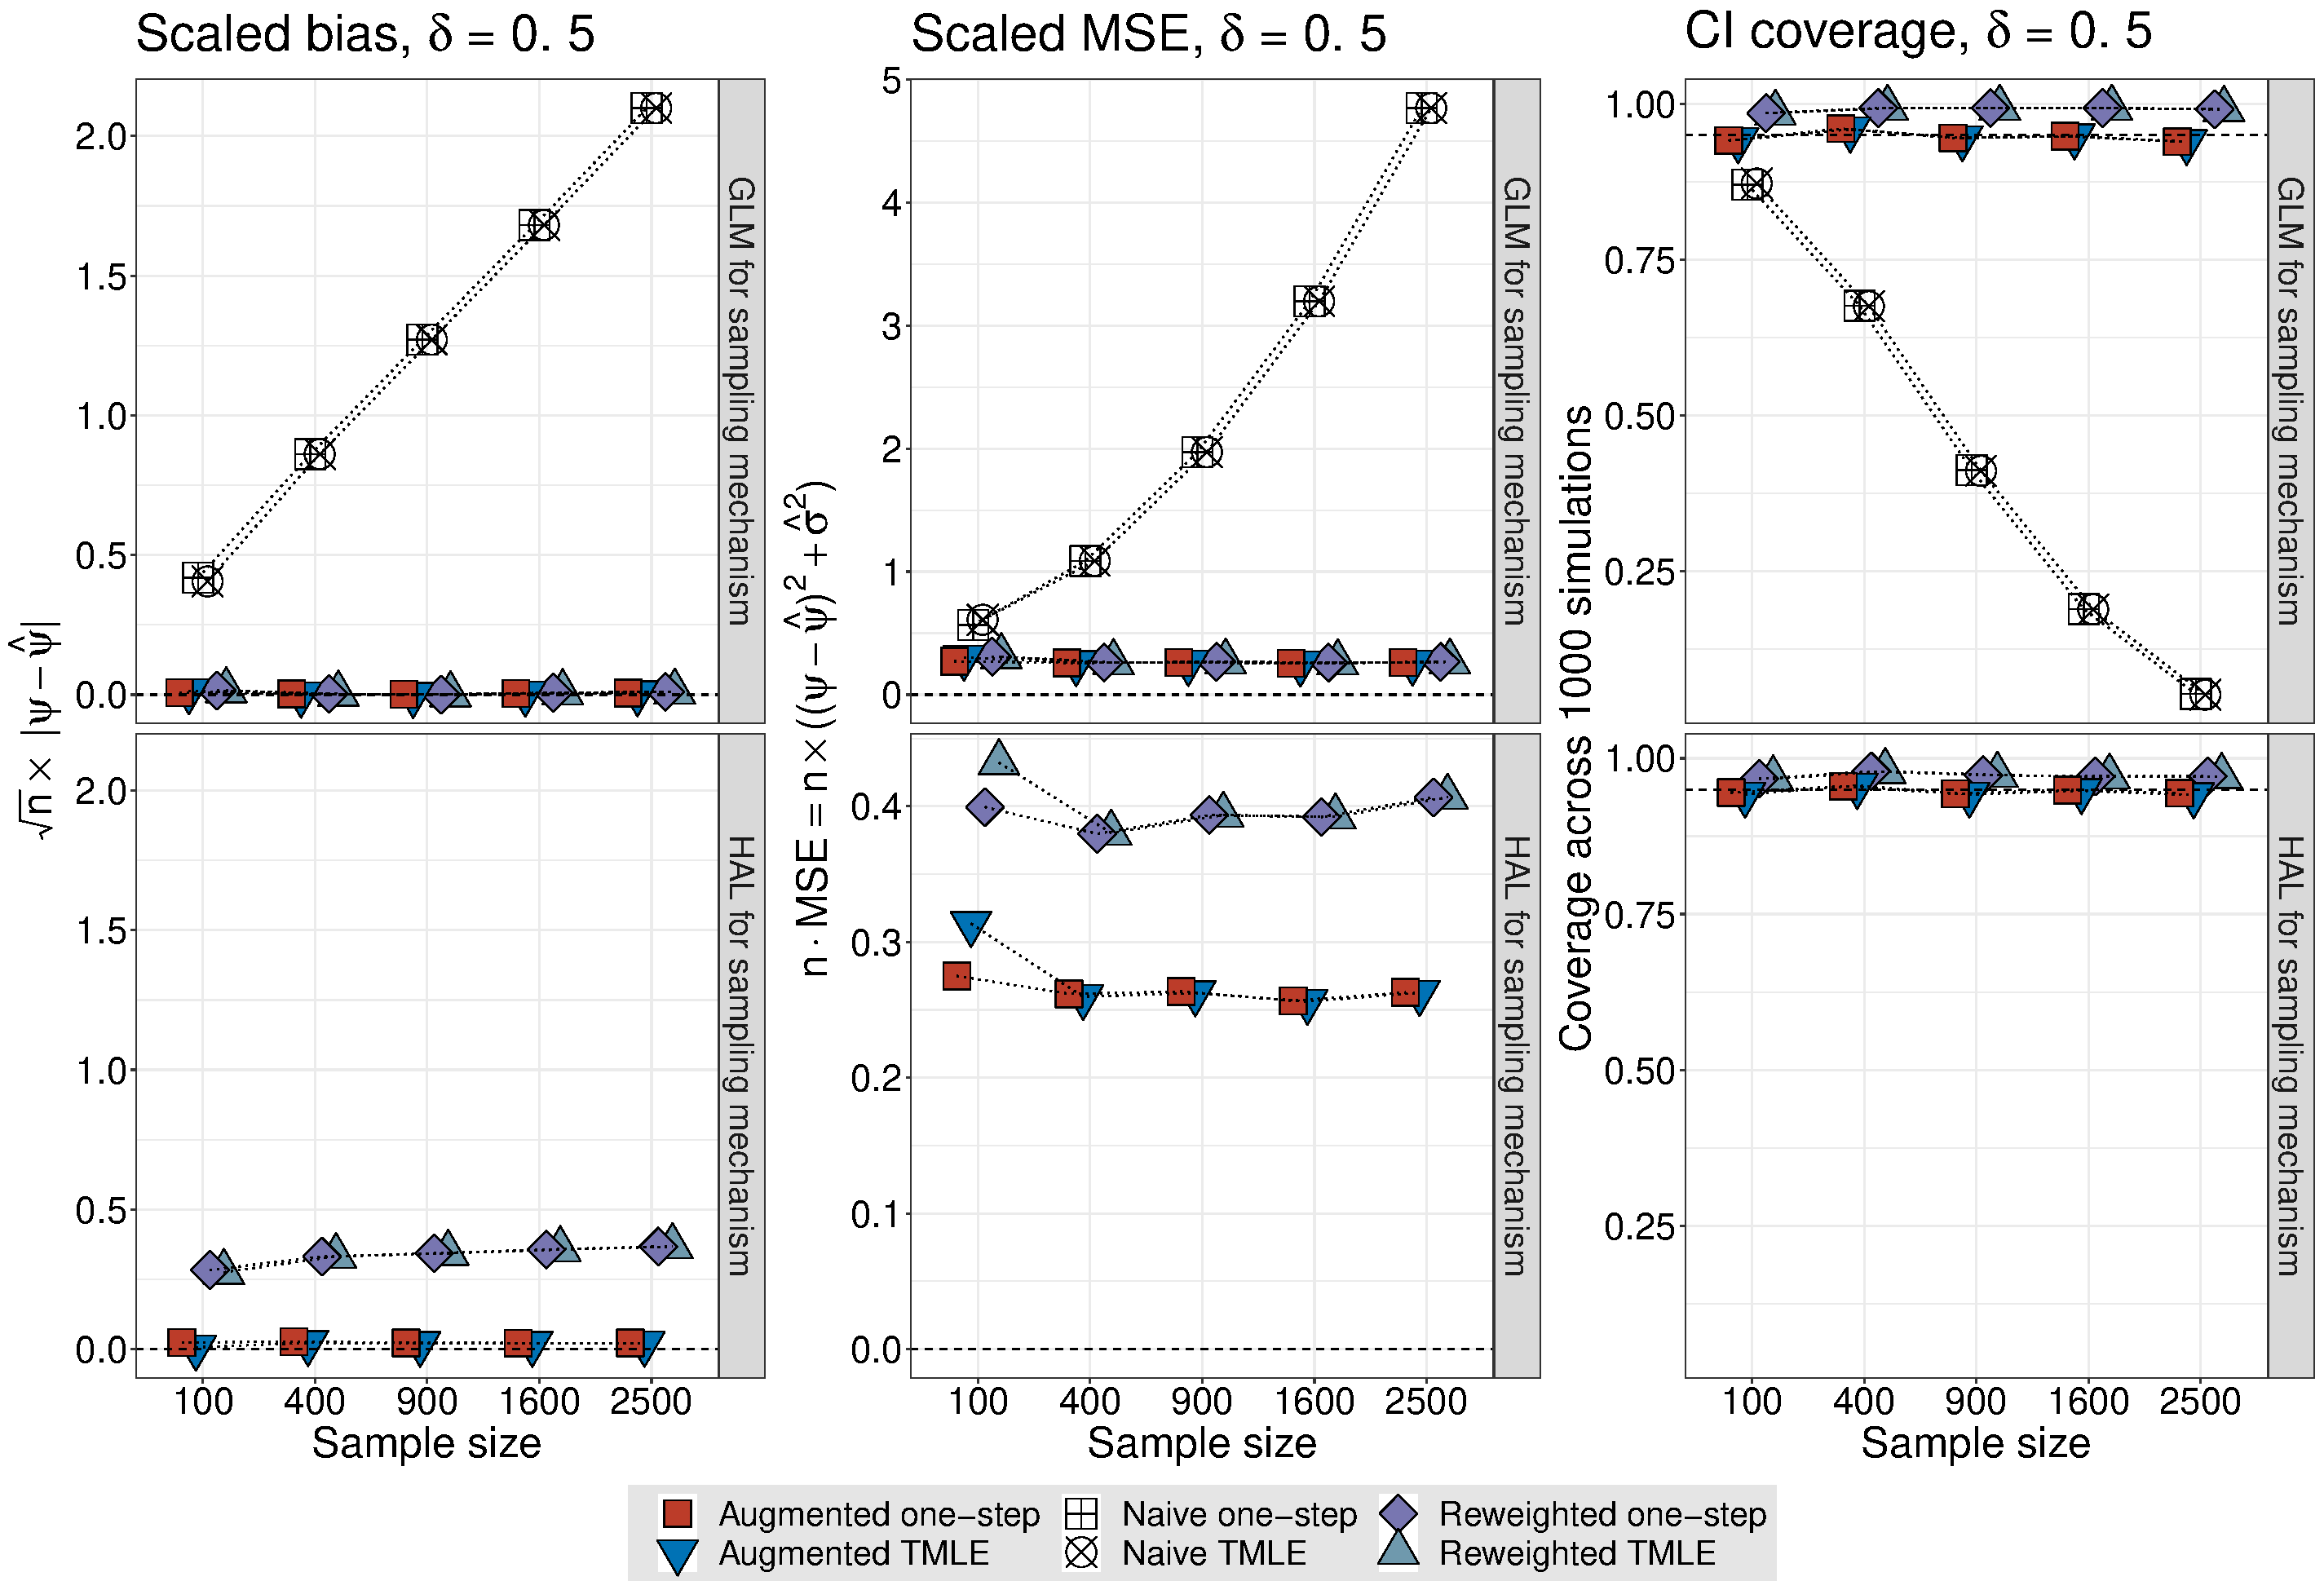
\includegraphics[scale=0.22]{simple_effect_panel_delta_upshift}
  \caption{
    Relative performance of reweighted and augmented estimators.
  }
\end{figure}

\note{
}

\end{frame}

%%%%%%%%%%%%%%%%%%%%%%%%%%%%%%%%%%%%%%%%%%%%%%%%%%%%%%%%%%%%%%%%%%%%%%%%%%%%%%%%

\begin{frame}[c]{A linear modeling perspective}

\begin{center}
\begin{itemize}
  \itemsep6pt
  \item Briefly consider a simple data structure: $X = (Y, A)$; we seek to model
    the outcome $Y$ as a function of $A$.
  \item To posit a linear model, consider $Y_i = \beta_0 + \beta_1 A_i +
    \epsilon_i$, with error $\epsilon_i \sim N(0, 1)$.
  \item Letting $\delta$ be a change in $A$, $Y_{A + \delta} - Y_A$ may be
    expressed
    \begin{align*}
      \E Y_{A + \delta} - \E Y_A &= [\beta_0 + \beta_1 (\E A + \delta)] -
        [\beta_0 + \beta_1 (\E A)] \\
        &= \beta_0 - \beta_0 + \beta_1 \E A - \beta_1 \E A + \beta_1 \delta \\
        &= \beta_1 \delta
    \end{align*}
  \item Thus, a \textit{unit shift} in $A$ (i.e., $\delta = 1$) may be seen as
    inducing a change in the difference in outcomes of magnitude $\beta_1$.
\end{itemize}
\end{center}

\note{
  \begin{itemize}
    \item We extend this result to the mean counterfactual outcomes under the
      nonparametric model $\M$.
    \item Linear modeling analogy re: conversation with Alan on 22 August.
  \end{itemize}
}

\end{frame}

%%%%%%%%%%%%%%%%%%%%%%%%%%%%%%%%%%%%%%%%%%%%%%%%%%%%%%%%%%%%%%%%%%%%%%%%%%%%%%%%

\begin{frame}[c]{A causal inference perspective}

\begin{center}
\begin{itemize}
  \itemsep6pt
  \item Consider a data structure: $(Y_a, a \in \mathcal{A})$.
  \item To posit a linear model, let $Y_a = \beta_0 + \beta_1 a
    + \epsilon_a$ for $a \in \mathcal{A}$, with error
    $\epsilon_a \sim N(0, \sigma^2_a)$ $\forall a \in A$.
  \item For the counterfactual outcomes $(Y_{a' + \delta}, Y_{a'})$, their
    difference, $Y_{a' + \delta} - Y_{a'}$, for some $a' \in \mathcal{A}$, may
    be expressed
    \begin{align*}
      \E Y_{a' + \delta} - \E Y_{a'} &= [\beta_0 + \beta_1 (a' + \delta) +
          \E \epsilon_{a' + \delta}] - [\beta_0 + \beta_1 a' +
          \E \epsilon_{a'}] \\
        &= \beta_1 \delta
    \end{align*}
  \item Thus, a \textit{unit shift} for $a' \in A$ (i.e., $\delta = 1$) may be
    seen as inducing a change in the difference in the counterfactual outcomes
    of magnitude $\beta_1$.
\end{itemize}
\end{center}

\note{
  \begin{itemize}
    \item Note that this analysis is exactly what we're told we \textbf{cannot}
      do in linear models 101 --- that is, the slope of a regression line cannot
      be interpreted as \textit{causing} a change in the outcome.
    \item We extend this result to the mean counterfactual outcomes under the
      nonparametric model $\M$.
    \item Linear modeling analogy re: conversation with Alan on 22 August.
    \item Example updated to incorporate countercatuals re: conversation with
      David on 30 August
  \end{itemize}
}

\end{frame}

%%%%%%%%%%%%%%%%%%%%%%%%%%%%%%%%%%%%%%%%%%%%%%%%%%%%%%%%%%%%%%%%%%%%%%%%%%%%%%%%

\begin{frame}[c]{Slope in a semiparametric model}

\begin{center}
\begin{itemize}
  \itemsep10pt
  \item Consider the stochastic intervention $g^{\star}(\cdot \mid L)$:
    \begin{align*}
      \E Y_{g^{\star}} &= \int_L \int_a \E(Y \mid A = a, L) g(a - \delta
            \mid L) \cdot da \cdot dP_0(L) \\
        &= \int_L \int_z \E(Y \mid A = z + \delta, L) g(z \mid L) \cdot dz
          \cdot dP_0(L),
    \end{align*}
      defning the change of variable $z = a - \delta$.
  \item For a semiparametric model, $\E (Y \mid A = z, L) = \beta z +
    \theta(L)$:
    \begin{align*}
      \E Y_{g^{\star}} - \E Y &= \int_L \int_z
      \begin{aligned}[t]
        & [\E(Y \mid A = z + \delta, L) - \E(Y \mid A = z, L)] \\
        & g(z \mid L) \cdot dz \cdot dP_0(L)
      \end{aligned} \\
      &= [\beta (z + \delta) + \theta(L)] - [\beta z + \theta(L)] \\
      &= \beta \delta
    \end{align*}
\end{itemize}
\end{center}

\note{
}

\end{frame}

%%%%%%%%%%%%%%%%%%%%%%%%%%%%%%%%%%%%%%%%%%%%%%%%%%%%%%%%%%%%%%%%%%%%%%%%%%%%%%%%

\begin{frame}[c]{Nonparametric conditional density estimation}

\begin{center}
\begin{itemize}
  \itemsep8pt
  \item To compute the auxiliary covariate $H(a,l)$, we need to estimate
    conditional densities $g(A \mid L)$ and $g(A - \delta \mid L)$.
  \item There is a rich literature on density estimation, we follow the approach
    proposed in \cite{diaz2011super}.
  \item To build a conditional density estimator, consider
    \begin{equation*}
      g_{n, \alpha}(a \mid L) = \frac{\pr (A \in [\alpha_{t-1}, \alpha_t)
        \mid L)}{\alpha_t - \alpha_{t-1}},
    \end{equation*}
    for $\alpha_{t-1} \leq a < \alpha_t$.
    \vspace{0.5em}
    \begin{itemize}
      \itemsep4pt
      \item This is a classification problem, where we estimate the probability
        that a value of $A$ falls in a bin $[\alpha_{t-1}, \alpha_t)$.
      \item The choice of the tuning parameter $t$ corresponds roughly to the
        choice of bandwidth in classical kernel density estimation.
    \end{itemize}
\end{itemize}
\end{center}

\note{
}

\end{frame}

%%%%%%%%%%%%%%%%%%%%%%%%%%%%%%%%%%%%%%%%%%%%%%%%%%%%%%%%%%%%%%%%%%%%%%%%%%%%%%%%

\begin{frame}[c]{Nonparametric conditional density estimation}

\begin{center}
\begin{itemize}
  \itemsep8pt
  \item \cite{diaz2011super} propose a re-formulation of this classification
    approach as a set of hazard regressions.
  \item To effectively employ this proposed re-formulation, consider
    \begin{align*}
      \pr (A \in [\alpha_{t-1}, \alpha_t) \mid L) =& \pr (A \in [\alpha_{t-1},
      \alpha_t) \mid A \geq \alpha_{t-1}, L) \times  \\ & \Pi_{j = 1}^{t -1}
      \{1 - \pr (A \in [\alpha_{j-1}, \alpha_j) \mid A \geq \alpha_{j-1}, L) \}
    \end{align*}
    \vspace{0.25em}
    \begin{itemize}
      \itemsep4pt
      \item The likelihood of this model may be expressed to correspond to the
        likelihood of a binary variable in a data set expressed via a long-form
        repeated measures structure.
      \item Specifically, the observation of $X_i$ is repeated as many times as
        intervals $[\alpha_{t-1}, \alpha_t)$ are before the interval to which
        $A_i$ belongs, and the binary variables indicating $A_i \in
        [\alpha_{t-1}, \alpha_t)$ are recorded.
    \end{itemize}
\end{itemize}
\end{center}

\note{
}

\end{frame}

%%%%%%%%%%%%%%%%%%%%%%%%%%%%%%%%%%%%%%%%%%%%%%%%%%%%%%%%%%%%%%%%%%%%%%%%%%%%%%%%

\begin{frame}[c]{Density estimation with the Super Learner algorithm}

\begin{center}
\begin{itemize}
  \itemsep10pt
  \item To estimate $g(A \mid L$) and $g(A - \delta \mid L)$, use a pooled
    hazard regression, spanning the support of $A$.
  \item We rely on the Super Learner algorithm of \cite{vdl2007super} to build
    an ensemble learner that optimally weights each of the proposed regressions,
    using cross-validation (CV).
  \item The Super Learner algorithm uses $V$-fold CV to train each proposed
    regression model, weighting each by the inverse of its average risk across
    all $V$ holdout sets.
  \item By using a library of regression estimators, we invoke the result of
    \cite{vdl2004asymptotic}, who prove this likelihood-based cross-validated
    estimator to be asymptotically optimal.
\end{itemize}
\end{center}

\note{
\begin{itemize}
  \item The auxiliary covariate simplifies when the treatment is in the limits
    (conditional on $L$) --- i.e., for $A_i \in (u(l) - \delta, u(l))$, then we
    have $H(a,l) = \frac{g_0(a - \delta \mid l)}{g_0(a \mid l)} + 1$.
  \item Asymptotically optimal in the sense that it performs as well as the
    oracle selector as the sample size increases.
\end{itemize}
}

\end{frame}

%%%%%%%%%%%%%%%%%%%%%%%%%%%%%%%%%%%%%%%%%%%%%%%%%%%%%%%%%%%%%%%%%%%%%%%%%%%%%%%%

% don't want dimming with references
\setbeamercovered{}
\beamerdefaultoverlayspecification{}

\begin{frame}[c,allowframebreaks]{}

\small
\bibliographystyle{apalike}
\nocite{*}
\bibliography{references}
%\itemize

\end{frame}

%%%%%%%%%%%%%%%%%%%%%%%%%%%%%%%%%%%%%%%%%%%%%%%%%%%%%%%%%%%%%%%%%%%%%%%%%%%%%%%%

\end{document}
